\documentclass{easychair}

\usepackage{doc}
\usepackage{graphicx}
\let\Bbbk\relax
\usepackage{latexsym,amsmath,amsfonts,amssymb,epsfig}
\usepackage{ifthen}
\usepackage{seqsplit}
\usepackage{url}
\usepackage{booktabs}
\usepackage{threeparttable}
\usepackage{adjustbox}
\usepackage{comment}

% --- Algorithm packages ---
% NOTE: We use `algorithm` + `algpseudocode` (algorithmicx) because
% the Step 1..Step 6 blocks use \State / \Return / \begin{algorithmic}.
% Do NOT load algorithm2e together with algpseudocode — they conflict.
\usepackage{algorithm}
\usepackage{algpseudocode}

\usepackage{color}
\usepackage{tabularx}
\usepackage{arydshln}
\usepackage{calc}
\usepackage{amstext}
\usepackage{multicol}
\usepackage{pslatex}
\usepackage{dashbox}
\usepackage{float}
\usepackage{inconsolata}
\usepackage{multirow}
\usepackage{makecell}
\usepackage{subcaption}
\usepackage{xcolor,listings}
\usepackage{enumitem}
\usepackage{placeins}
\usepackage{pgfplots}
\pgfplotsset{compat=1.18}
\usetikzlibrary{patterns}

% --- Custom macros ---
\newcommand{\Hf}{\mathsf{H}}
\newcommand{\HkdfExtract}{\mathsf{HKDF\text{-}Extract}}
\newcommand{\HkdfExpand}{\mathsf{HKDF\text{-}Expand}}
\newcommand{\KDF}{\mathsf{KDF}}
\newcommand{\DHf}{\mathsf{DH}}
\newcommand{\AEnc}{\mathsf{Enc}}
\newcommand{\ADec}{\mathsf{Dec}}
\newcommand{\KemKeyGen}{\mathsf{KeyGen}}

% --- Variant naming macros (uniform "Section X.Y~\cite{pq-edhoc-draft}") ---
% Use \VarSec{2} or \VarSec{3.2} ... in body text whenever you refer to a
% variant of the proposed protocol. This guarantees a single, uniform style
% paper-wide and makes future edits trivial.
\newcommand{\VarSec}[1]{Section~#1~\cite{pq-edhoc-draft}}
% Short variant (no citation), useful inside captions/tables where the
% citation would already have been introduced or is redundant:
\newcommand{\VarSecShort}[1]{Section.~#1}

\usepackage[
    n, operators, advantage, sets, adversary, landau, probability,
    notions, logic, ff, mm, primitives, events, complexity,
    asymptotics, keys]{cryptocode}

\sloppy
\renewcommand{\arraystretch}{1.3}

\newcommand{\EDHOC}{\textsf{EAP-EDHOC-PQ}}
\newcommand{\Hash}{\sf{H}}
\newcommand{\Code}[1]{\ttfamily #1}
\newcommand{\HKDFextract}{\mathrm{HKDF\text{-}Extract}}
\newcommand{\HMAC}{\mathrm{HMAC\text{-}SHA256}}
\newcommand{\SHA}{\mathrm{SHA256}}
\newcommand{\X}{\mathsf{X25519}}
\newcommand{\Encaps}{\mathsf{KEM.Encaps}}
\newcommand{\Decaps}{\mathsf{KEM.Decaps}}
\newcommand{\Ed}{\mathsf{Ed25519}}
\newcommand{\CBOR}{\mathsf{CBOR}}
\newcommand{\Concat}{\mathbin{\|}}

\title{EAP-EDHOC-PQC: Quantum-Safe Onboarding for IoT E-Business Beyond Extensible Authentication Protocol}

\author{
Adi Panca Saputra Iskandar\inst{1,2}
\and
I Wayan Adi Juliawan Pawana\inst{1,2}
\and
Ilsun You\inst{2}
}

\institute{
Kookmin University, Seoul, Korea\\
\email{adipancaiskandar@gmail.com, adijuliawanpawana@unud.ac.id, ilsunu@gmail.com}
\and
Udayana University, Bali, Indonesia\\
}

\authorrunning{Iskandar et al.}
\titlerunning{EAP-EDHOC-PQC}

\begin{document}

\maketitle

\begin{abstract}
The Internet of Things (IoT) underpins a growing range of e-business
operations networked vending machines, smart point-of-sale and
self-checkout terminals, electronic shelf labels, smart-retail
beacons, electric-vehicle (EV) chargers, smart parking meters, fleet
and cold-chain trackers, and industrial sensor gateways all of
which onboard onto Wi-Fi or other non-3GPP networks via the
Extensible Authentication Protocol (EAP) and must remain secure
against a future quantum adversary. Ephemeral Diffie--Hellman over
COSE (EDHOC, RFC~9528) is a lightweight authenticated key exchange
for constrained devices, and the Internet-Draft
\texttt{draft-papon-lake-pq-edhoc} defines five post-quantum (PQ)
authentication variants over ML-KEM and ML-DSA. The combined impact
of PQ key enlargement, EAP fragmentation, and RADIUS transport on a
real AAA deployment, however, has not yet been quantified, and
formal analyses of the PQ-EDHOC variants integrated with EAP are
scarce. We close these gaps by proposing \emph{EAP-EDHOC-PQ}, a
unified EAP method that embeds all five PQ-EDHOC variants. We verify
mutual authentication, session-key secrecy, forward secrecy, and
replay resistance under a Dolev--Yao adversary in ProVerif, and we
empirically evaluate the design on a heterogeneous IoT testbed
(Raspberry~Pi~5 Initiator, MacBook~Air~M3 Authenticator/Responder)
across three deployments: Non-EAP, EAP-Standalone, and full
EAP/RADIUS with FreeRADIUS. At a conservative 256-byte fragment
size, total wire bytes range from $7{,}031$ to $11{,}614$ ($29$ to
$48$ fragments) and AAA-path handshake time from $56$~ms to $440$~ms
across variants. A first-order energy model derived from the same
measurements shows that fragment-induced I/O wait not
cryptography dominates the per-handshake energy of an IoT-class
endpoint. The results quantify the trade-off between authentication
strength, round-trip count, and fragmentation, and give concrete
deployment guidance for PQ network-access authentication in
e-business IoT settings.

\flushleft{{\bf Keywords:} E-Business Security, IoT, EDHOC, EAP,
Post-Quantum Cryptography, ML-KEM, ML-DSA, ProVerif, FreeRADIUS}
\end{abstract}


%=========================================================================
\section{Introduction}
\label{Introduction}
%=========================================================================
IoT is increasingly embedded in everyday e-business workflows.
Representative business-critical endpoints include
\emph{(i)}~networked vending machines accepting cashless and QR-code
payments;
\emph{(ii)}~smart point-of-sale (POS) and self-checkout terminals;
\emph{(iii)}~electronic shelf labels and smart-retail beacons that
drive in-store engagement;
\emph{(iv)}~EV chargers and smart parking meters operated by retail
or city operators;
\emph{(v)}~fleet trackers and cold-chain sensors monitoring logistics
conditions; and
\emph{(vi)}~connected industrial sensors and programmable
logic-controller (PLC) gateways feeding predictive-maintenance
pipelines on the factory floor.
Each of these devices is, in commercial terms, a small business
endpoint that handles payment data, customer behaviour, or
operational telemetry, and must therefore be enrolled and
authenticated before exchanging data with the back-office. As such
endpoints onboard onto enterprise networks --- most often via Wi-Fi
or other non-3GPP access --- \emph{network access authentication} is
the first line of defence that establishes device identity, derives
session keys, and gates the device onto production traffic. EAP~\cite{RFC3748}
provides the dominant framework for this task: it is used by
IEEE~802.1X, Wi-Fi WPA2/3-Enterprise, and 5G-AKA, and it typically
runs over a RADIUS/Diameter backend in which a central
Authentication, Authorization and Accounting (AAA) server makes the
final authentication decision.

Among the many EAP methods, EAP-TLS~\cite{RFC5216}, EAP-AKA~\cite{RFC4187}
and EAP-PSK~\cite{RFC4764} are the most widely deployed. For constrained
IoT devices, however, EAP-TLS is expensive in bytes on the wire and
certificate chains~\cite{FVW24,LopezGomez2026}. EDHOC~\cite{RFC9528,RFC9529}
is a lightweight authenticated Diffie--Hellman key exchange using
Concise Binary Object Representation (CBOR)~\cite{RFC8949} and
CBOR Object Signing and Encryption (COSE)~\cite{RFC9052}, designed
for constrained networks and standardized by the IETF LAKE working
group~\cite{LAKE}. Recent work proposes embedding EDHOC as an EAP
method~\cite{RFC-EAP-EDHOC,LopezGomez2026}, which brings EDHOC's
compact flights to mainstream AAA-based network access.

At the same time, Shor's algorithm~\cite{shor1994algorithms} threatens
every elliptic-curve deployment in use today. While a
cryptanalytically relevant quantum computer is not yet available, the
\emph{harvest-now, decrypt-later} adversary model is already a
documented concern for long-lived business data such as payment
records and supply-chain telemetry, and motivates beginning the
transition before such a machine appears. NIST has standardized ML-KEM
(FIPS~203)~\cite{FIPS203} and ML-DSA (FIPS~204)~\cite{FIPS204} as
first-line post-quantum replacements. Regulators
in France~\cite{ANSSI} and Germany~\cite{TR-02102-1} and the IETF PQUIP working
group~\cite{PQUIP} recommend \emph{hybrid} PQ/traditional combinations during
the transition period. A post-quantum variant of EDHOC
(\texttt{draft-papon-lake-pq-edhoc}) is under active
specification~\cite{pq-edhoc-draft} and defines five authentication modes
in its Sections~2, 3.2, 3.3, 3.4 and 3.5; follow-up analyses have evaluated
quantum-resistant EDHOC on microcontrollers~\cite{FTK+25,FKF25}.

What is not yet understood is what happens when these PQ-EDHOC variants are
carried by \emph{EAP in a real AAA setting}. EAP defines a minimum
MTU of only 1020 octets and mandates a lock-step, fragment-ACK flow for
payloads larger than that~\cite{RFC3748,RFC9191}. ML-KEM ciphertexts and
ML-DSA signatures push individual EDHOC messages into the multi-kilobyte
range, so each handshake message incurs multiple fragments and additional
round-trips end-to-end between the EAP peer, the authenticator, and the
AAA server. Prior empirical EDHOC studies~\cite{FVW24,FTK+25,FKF25}
evaluated EDHOC peer-to-peer and did not exercise an EAP/RADIUS path; prior
EAP-EDHOC work~\cite{RFC-EAP-EDHOC,LopezGomez2026} has focused on the
classical primitive set.

% \subsection{Related Work}
% \label{sec:related-work}
Our work sits at the intersection of four threads: (i) the EAP framework
itself and its canonical methods~\cite{RFC3748,RFC5216,RFC4187,RFC4764};
(ii) EDHOC and its integration with EAP~\cite{RFC9528,RFC9529,LAKE,RFC-EAP-EDHOC,LopezGomez2026,FVW24};
(iii) post-quantum and hybrid key exchange, including FIPS~203/204~\cite{FIPS203,FIPS204},
ETSI TS~103~744~\cite{TS103744}, PQXDH~\cite{PQXDH,FG24}, PQ
Noise~\cite{ADH+22}, hybrid IKEv2~\cite{RFC9370}, and hybrid
TLS~1.3~\cite{TLS}; and (iv) formal and computational analyses of EDHOC such
as~\cite{KDL+21,NSB21,CP22,GM23,JKK+23,Fer24,PSM+24}. The KEM-based
EDHOC authentication Internet-Draft~\cite{pocero} and the
signature/KEM PQ-EDHOC draft~\cite{pq-edhoc-draft} are the closest
antecedents to our proposal, and stronger KEM notions such as those in
\cite{CDM24} motivate why KEM-authenticated handshakes deserve careful
symbolic treatment. Despite substantial progress in each of these threads, four gaps remain. \emph{First}, the impact of PQ key/ciphertext enlargement on EAP fragmentation under the minimum 1020-octet EAP MTU has not been quantified. \emph{Second}, formal symbolic analyses of the PQ variants of EAP-EDHOC have not been published, and existing ProVerif models target classical EDHOC~\cite{NSB21,JKK+23}. \emph{Third}, empirical evaluations of PQ-EDHOC have so far targeted EDHOC peer-to-peer or microcontrollers without a real AAA backend~\cite{FTK+25,FKF25}. \emph{Fourth}, the different PQ-EDHOC authentication modes (KEM-only, signature-only, and hybrid) have not been compared uniformly in a deployment with EAP and a real AAA server such as FreeRADIUS.

\subsection{Contribution}
\label{sec:contribution}
We address these gaps with the following contributions. Throughout the
paper we refer to the five authentication variants of
\texttt{draft-papon-lake-pq-edhoc} by their draft-section numbers,
namely \VarSec{2}, \VarSec{3.2}, \VarSec{3.3}, \VarSec{3.4} and
\VarSec{3.5}; this nomenclature is used uniformly in every algorithm,
table, and figure of the paper.
\begin{itemize}[leftmargin=1.2em,itemsep=2pt,topsep=2pt]
\item We specify EAP-EDHOC-PQ, a unified EAP method that embeds
the five PQ-EDHOC authentication variants of~\cite{pq-edhoc-draft} ---
the implicitly KEM-authenticated three-flight mode (\VarSec{2},
Section~\ref{sec:variant-s2}); the signature+KEM three-flight mode
(\VarSec{3.2}, Section~\ref{sec:variant-s32}); and three four-flight
hybrid variants (\VarSec{3.3}, \VarSec{3.4} and \VarSec{3.5},
Sections~\ref{sec:variant-s33}--\ref{sec:variant-s35}) over EAP and
RADIUS.
\item We provide a ProVerif model of all five variants and prove
mutual authentication, session-key secrecy, forward secrecy, and replay
resistance under a Dolev--Yao adversary
(Section~\ref{security-analysis}).
\item We provide an empirical evaluation on a real testbed with
Non-EAP, EAP-Standalone, and full EAP/RADIUS (FreeRADIUS) deployments at
a conservative 256-byte fragment size, measuring fragmentation,
processing time, overhead, and per-operation latency
(Section~\ref{performance-evaluation}).
\item We derive concrete deployment guidance: which variant
minimizes wire bytes, which minimizes round-trips, and how the AAA path
amplifies the cost of four-flight hybrid modes
(Section~\ref{discussion}).
\end{itemize}

The remainder of the paper is organized as follows.
Section~\ref{pleminary} introduces the primitives, the EAP/RADIUS model,
and notation. Section~\ref{proposed-design} specifies the unified
EAP-EDHOC-PQ design and its five variants.
Section~\ref{sec:comparison} compares our unified design with the
original two-mode presentation of~\cite{pq-edhoc-draft}.
Section~\ref{security-analysis} presents the ProVerif analysis.
Section~\ref{performance-evaluation} reports the empirical evaluation.
Section~\ref{discussion} discusses implications and limitations.
Section~\ref{conclusion} concludes.


%=========================================================================
\section{Preliminaries}
\label{pleminary}
%=========================================================================
This section fixes notation, recalls the cryptographic primitives we use,
summarizes EDHOC and EAP, and introduces the
threat model. Table~\ref{tab:abbr} lists the abbreviations used
throughout the paper.

\begin{table}[h]
\centering
\scriptsize
\caption{Abbreviations and notation used throughout the paper
(including all symbols of Algorithms~\ref{alg:step1}--\ref{alg:step6}
in Section~\ref{proposed-design}).}
\label{tab:abbr}
\setlength{\tabcolsep}{4pt}
\begin{tabularx}{\linewidth}{@{}l X l X@{}}
\toprule
\textbf{Symbol} & \textbf{Description} & \textbf{Symbol} & \textbf{Description} \\
\midrule
\multicolumn{4}{l}{\textit{Protocols and frameworks}} \\
EAP    & Extensible Authentication Protocol (RFC~3748) & EDHOC  & Ephemeral Diffie--Hellman over COSE (RFC~9528) \\
AAA    & Authentication, Authorization, Accounting (RADIUS/Diameter) & NAS    & Network Access Server (relays EAP between peer and AAA) \\
RADIUS & Remote Authentication Dial-In User Service (RFC~2865) & CBOR   & Concise Binary Object Representation (RFC~8949) \\
COSE   & CBOR Object Signing and Encryption (RFC~9052) & MTU    & Maximum Transmission Unit \\
LAKE   & IETF working group for Lightweight AKE & & \\
\midrule
\multicolumn{4}{l}{\textit{Cryptographic primitives}} \\
KEM    & Key Encapsulation Mechanism & ML-KEM & Module-Lattice KEM (FIPS~203) \\
ML-DSA & Module-Lattice Digital Signature Algorithm (FIPS~204) & DS     & Digital Signature scheme (instantiated by ML-DSA) \\
AEAD   & Authenticated Encryption with Associated Data & HKDF   & HMAC-based Extract-and-Expand KDF (RFC~5869) \\
KDF    & Key Derivation Function & HMAC   & Hashed Message Authentication Code \\
MAC    & Message Authentication Code & SHA-256 & Secure Hash Algorithm, 256-bit output \\
$H(\cdot)$ & cryptographic hash (SHA-256 in our instantiation) & $\KemKeyGen,\Encaps,\Decaps$ & KEM key generation, encapsulation, decapsulation \\
$\mathbf{DS.Sign},\mathbf{DS.Verify}$ & digital-signature signing / verification & $\mathbf{AEAD.Enc},\mathbf{AEAD.Dec}$ & AEAD encryption / decryption \\
\midrule
\multicolumn{4}{l}{\textit{Parties, identifiers and credentials}} \\
$I$, $R$ & EDHOC Initiator, Responder & $C_I$, $C_R$ & EDHOC connection identifiers chosen by $I$, $R$ \\
$ID\_CRED_I$, $ID\_CRED_R$ & credential identifier of $I$, $R$ & METHOD, $\mathrm{SUITES}_I$ & EDHOC method byte and offered cipher-suite list \\
$\mathrm{EAD}_i$ & External Authorization Data field of message~$i$ & MSK, EMSK & Master Session Key, Extended MSK exported to EAP \\
\midrule
\multicolumn{4}{l}{\textit{Per-handshake key material}} \\
$sk_X, pk_X$ & long-term secret/public key of party $X$ & $\mathrm{kem.sk}_X, \mathrm{kem.pk}_X$ & long-term KEM key pair of party $X$ \\
$\mathrm{sign.sk}_X, \mathrm{sign.pk}_X$ & long-term signing key pair of party $X$ & $\mathrm{kem.sk}_{\mathrm{eph}}, \mathrm{kem.pk}_{\mathrm{eph}}$ & ephemeral KEM key pair generated by $I$ \\
$\mathrm{kem.ct}_{\mathrm{eph}}$ & KEM ciphertext encapsulating to $\mathrm{kem.pk}_{\mathrm{eph}}$ & $\mathrm{kem.ct}_R, \mathrm{kem.ct}_I$ & KEM ciphertexts encapsulating to $R$'s, $I$'s long-term key \\
$\mathrm{ss}_{\mathrm{eph}}, \mathrm{ss}_R, \mathrm{ss}_I$ & shared secrets from the three KEM operations & $TH_i$ & EDHOC transcript hash after message~$i$ \\
$PRK_{2e}$ & PRK from $\mathrm{ss}_{\mathrm{eph}}$ & $PRK_{3e2m}$ & PRK after mixing $\mathrm{ss}_R$ \\
$PRK_{4e3m}$ & PRK after mixing $\mathrm{ss}_I$ (four-flight modes) & $PRK_{\mathrm{out}}$ & exporter PRK feeding MSK/EMSK derivation \\
$SALT_{3e2m}, SALT_{4e3m}$ & salts used in the corresponding HKDF-Extract & $KEYSTREAM_2$ & XOR keystream protecting $PLAINTEXT_2$ \\
$K_3,IV_3,K_4,IV_4$ & AEAD key/IV pairs for messages 3 and 4 & $MAC_i$ & authentication tag carried in (or covering) flight~$i$ \\
$SIGNATURE_i$ & ML-DSA signature attached to flight~$i$ & $PLAINTEXT_i, CIPHERTEXT_i$ & plaintext / ciphertext payload of message~$i$ \\
$\parallel$ & byte-string concatenation & & \\
\bottomrule
\end{tabularx}
\end{table}

% \subsection{Cryptographic Primitives}
We use NIST-standardized post-quantum primitives.
\textbf{ML-KEM}~\cite{FIPS203} is an IND-CCA2-secure key-encapsulation
mechanism with three algorithms $(\KemKeyGen,\Encaps,\Decaps)$.
\textbf{ML-DSA}~\cite{FIPS204} is a module-lattice digital signature
algorithm. Symmetric primitives follow RFC~9528: SHA-256 for hashing,
HKDF~\cite{RFC5869} for key derivation, and AES-CCM (an AEAD) for
authenticated encryption.

% \subsection{EDHOC (RFC 9528)}
EDHOC is a three-message (optionally four-message) authenticated key
exchange encoded in CBOR~\cite{RFC8949,RFC9052}. The canonical
Signature-Signature (SIG-SIG) method transmits ephemeral Diffie--Hellman
contributions and authenticates both parties with digital signatures; the
Static-DH modes use long-term DH keys and derive MAC tags instead.
A detailed security analysis in the classical setting is provided
in~\cite{NSB21,CP22,GM23,JKK+23,Fer24,PSM+24}.

% \subsection{EAP and RADIUS Model}
EAP~\cite{RFC3748} is a lock-step request/response protocol operating over
a lower layer (e.g., IEEE~802.1X, PPP, or IKEv2). For EAP-over-RADIUS, an
\emph{authenticator} (typically a gateway or access point) relays EAP
packets between the peer and the AAA server inside RADIUS attributes. Two
properties are central to our evaluation. \emph{(a)} EAP implementations
may assume an MTU of only 1020 octets from the lower layer, and EAP itself
does not provide fragmentation; an EAP method whose messages exceed the
MTU must implement fragmentation with explicit ACKs, at the cost of extra
round-trips~\cite{RFC3748,RFC9191}. \emph{(b)} RADIUS packets are capped
at 4096 octets and carry EAP payloads in multiple \texttt{EAP-Message}
AVPs of 253 bytes each; long EAP messages therefore cross both the EAP
fragmentation boundary and the RADIUS attribute boundary.

% \subsection{Threat Model}
We consider a Dolev--Yao adversary~\cite{dolev1983security} controlling the
network between the peer, the authenticator, and the AAA server. The
adversary may inject, drop, reorder, replay, or modify any message and may
corrupt long-term keys of peers other than the target session for forward
secrecy arguments. Cryptographic primitives are idealized as perfect
symbolic functions, consistent with ProVerif's applied-pi-calculus model
and standard practice~\cite{blanchet2001proverif,blanchet2016automated,cremers2017symbolic}.


%=========================================================================
\section{Proposed Design: EAP-EDHOC-PQ}
\label{proposed-design}
%=========================================================================
The proposed \textbf{EAP-EDHOC-PQ} method carries PQ-EDHOC flights between
the EAP peer (the EDHOC Initiator $I$, typically an IoT device), the
authenticator, and the AAA server (the EDHOC Responder $R$). The unified
design supports five authentication variants --- \VarSec{2},
\VarSec{3.2}, \VarSec{3.3}, \VarSec{3.4}, and \VarSec{3.5} --- that
trade off the authentication mechanism (KEM, signature, or hybrid),
the number of flights (three or four), and the timing of responder
authentication. Figure~\ref{fig:protocol} summarizes the complete
protocol flow. Sections~\ref{sec:variant-s2}--\ref{sec:variant-s35}
describe the variants individually. Common header (EAP Identity and EDHOC-Start). All variants begin with the standard EAP Identity exchange: the
authenticator relays the peer's EAP-Response/Identity to the AAA server,
which answers with a RADIUS Access-Challenge carrying
EAP-Request/EDHOC-Start. From this point on the five variants diverge.

\subsection{Variant 1 \texorpdfstring{\VarSec{2}}{Section 2 of the draft}}
\label{sec:variant-s2}
\VarSec{2} authenticates the Initiator explicitly with an ML-DSA
signature and the Responder \emph{implicitly} through ML-KEM, following
the philosophy of~\cite{pocero}. Before the handshake the Initiator
knows the Responder's long-term KEM public key $\mathit{kem.pk}_R$.
Message\,1 carries an ephemeral KEM public key
$\mathit{kem.pk}_{\mathit{eph}}$ together with the static-to-Responder
ciphertext $\mathit{kem.ct}_R \leftarrow \Encaps(\mathit{kem.pk}_R)$,
which delivers $\mathit{ss}_R$ to the Responder. The Responder then
encapsulates to the Initiator's ephemeral KEM key, producing
$(\mathit{ss}_{\mathit{eph}},\mathit{kem.ct}_{\mathit{eph}})$, and mixes
both shared secrets into $\mathit{PRK}_{\mathit{3e2m}} =
\HKDFextract(\mathit{SALT}_{\mathit{3e2m}},\mathit{ss}_R)$. The
Responder is authenticated by its ability to decapsulate
$\mathit{ss}_R$, which is the MAC key that Message\,3 verifies.
Message\,4 is optional (key confirmation only). This variant is the
smallest on the wire and uses a single KEM decapsulation at $R$ per
handshake.

\subsection{Variant 2 \texorpdfstring{\VarSec{3.2}}{Section 3.2 of the draft}}
\label{sec:variant-s32}
\VarSec{3.2} provides explicit Responder authentication via ML-DSA in
Message\,2 while still achieving a three-flight main handshake.
Message\,1 carries only $\mathit{kem.pk}_{\mathit{eph}}$; the Responder
encapsulates to it and signs $PLAINTEXT_2$ with its ML-DSA key. The
Initiator encapsulates to $\mathit{kem.pk}_R$ in Message\,3, delivering
$\mathit{ss}_R$ to the Responder and binding the handshake to the
Responder's long-term KEM identity. Compared with \VarSec{2},
\VarSec{3.2} replaces the implicit KEM authentication of $R$ with an
explicit signature in Message\,2 and therefore pays a larger Message\,2
on the wire.

\subsection{Variant 3 \texorpdfstring{\VarSec{3.3}}{Section 3.3 of the draft}}
\label{sec:variant-s33}
\VarSec{3.3} is the \emph{mirror} of \VarSec{3.2} with respect to the
direction of the static KEM. Authentication of $I$ uses both an ML-DSA
signature and KEM confirmation \emph{to the Initiator}, so the Responder
must encapsulate to $\mathit{kem.pk}_I$ after learning
$\mathit{ID\_CRED}_I$ in Message\,3. This forces Message\,4 to become
\emph{mandatory}: it carries $\mathit{kem.ct}_I$ and the encrypted
confirmation. \VarSec{3.3} therefore yields a four-flight handshake,
with the natural cost that the AAA path adds one more RADIUS
round-trip.

\subsection{Variant 4 \texorpdfstring{\VarSec{3.4}}{Section 3.4 of the draft}}
\label{sec:variant-s34}
\VarSec{3.4} implements KEM+KEM authentication on both sides but defers
Responder authentication: the Responder's MAC tag is not sent in
Message\,2 but carried inside Message\,4, after $R$ has encapsulated to
$\mathit{kem.pk}_I$. The design yields three shared secrets
$\{\mathit{ss}_{\mathit{eph}},\mathit{ss}_R,\mathit{ss}_I\}$ and the
strongest key-contributiveness among our variants, at the cost of one
additional KEM operation on each side.

\subsection{Variant 5 \texorpdfstring{\VarSec{3.5}}{Section 3.5 of the draft}}
\label{sec:variant-s35}
\VarSec{3.5} combines the best of the hybrid options: explicit ML-DSA
authentication of $R$ in Message\,2 \emph{and} KEM-based authentication
of $I$ via Message\,4. It is the ``full hybrid'' variant and provides
the strongest authentication guarantees in our family at the cost of
the highest wire size and the most cryptographic operations.

% \subsection{Fragmentation and AEAD framing}
Every EDHOC message is carried inside an EAP-Request/EAP-Response of
type \texttt{EAP-EDHOC-PQ}. When the EAP payload exceeds the negotiated
fragment size, EAP-EDHOC-PQ uses an explicit flag-based fragmentation
with \texttt{M}-bit (``more fragments''), mirroring EAP-TLS and the
classical EAP-EDHOC draft~\cite{RFC-EAP-EDHOC,LopezGomez2026}. Each
fragment carries a 4-byte EAP header; the sender waits for an ACK
fragment (an EAP-Response of type EAP-EDHOC-PQ with empty data) before
sending the next fragment, introducing one lock-step round-trip per
fragment pair.
%=========================================================================
% \subsection{Comparison with Related Designs}
% \label{sec:comparison}
%=========================================================================
The original PQ-EDHOC Internet-Draft~\cite{pq-edhoc-draft} groups its
five variants under two umbrella modes (SIG-SIG and MAC-MAC) and
develops the SIG-SIG mode as a single Section~3.2 example, without
any consideration of EAP transport. Closely related work either keeps
EDHOC peer-to-peer over UDP/CoAP~\cite{FTK+25,FKF25,FVW24} or embeds
\emph{classical} EDHOC into EAP~\cite{RFC-EAP-EDHOC,LopezGomez2026}.
No prior design carries all five PQ-EDHOC variants over a real
EAP/RADIUS path with an off-the-shelf AAA server, and prior
comparisons therefore cannot speak to the cost of EAP fragmentation,
the RADIUS attribute boundary, or the lock-step ACK round-trip. Our
unified specification fills this gap. \VarSec{2} is the only mode
that retains the three-flight structure \emph{and} drops one signature
relative to SIG-SIG, while \VarSec{3.4} is, to the best of our
knowledge, the first EAP-friendly KEM+KEM hybrid with deferred
Responder authentication suitable for fragmentation under the EAP
MTU.
Two dimensions distinguish our design from the alternatives.
\emph{First, EAP transport vs.\ peer-to-peer.} A peer-to-peer
PQ-EDHOC handshake travels over a single UDP/CoAP~\cite{RFC9528}
association between $I$ and $R$, with no fragmentation contract
beyond what the lower layer offers; in contrast, EAP imposes a
lock-step request/response state machine, an MTU as low as $1020$
octets~\cite{RFC3748,RFC9191}, and a fragment-ACK exchange that adds
one round-trip per fragment pair. The same multi-kilobyte ML-DSA
signature therefore costs proportionally more wall-clock time on EAP
than in a peer-to-peer setting a cost that is invisible from the
draft's own description.
\emph{Second, AAA backend vs.\ standalone.} An EAP-Standalone
deployment terminates EAP at the authenticator, while a full AAA
deployment relays each EAP message inside RADIUS
\texttt{EAP-Message} attributes (capped at $253$ bytes
each~\cite{RFC2865}) over a separate Network Access
Server~$\leftrightarrow$~AAA hop. The RADIUS hop adds latency but
also amortizes some I/O via FreeRADIUS's batched packetization, and
the joint behaviour cannot be inferred from the peer-to-peer numbers
alone.

% ============================================
% STEP 1: INITIATOR — Prepare Message 1
% ============================================
\begin{algorithm}[H]
\caption{Step 1 (Initiator) --- Prepare $M_1$}
\label{alg:step1}
\textbf{Input:} Longterm PQ key pair $(pk_I, sk_I)$; Responder's $\mathrm{kem.pk}_R$ (Section~2 only) \\
\textbf{Output:} $M_1$
\begin{algorithmic}[1]
\Statex \textit{[All Sections]}
\State $(\mathrm{kem.sk}_{\mathrm{eph}}, \mathrm{kem.pk}_{\mathrm{eph}}) \gets \mathbf{KEM.KeyGen}()$
\Statex \textit{[Section 2 only]}
\State $(\mathrm{ss}_R, \mathrm{kem.ct}_R) \gets \mathbf{KEM.Encaps}(\mathrm{kem.pk}_R)$
\State $M_1 \gets (\mathrm{METHOD}, \mathrm{SUITES}_I, \mathrm{kem.pk}_{\mathrm{eph}}, \mathrm{kem.ct}_R, C_I, \mathrm{EAD}_1)$
\Statex \textit{[Section 3.2, 3.3, 3.4, 3.5]}
\State $M_1 \gets (\mathrm{METHOD}, \mathrm{SUITES}_I, \mathrm{kem.pk}_{\mathrm{eph}}, C_I, \mathrm{EAD}_1)$
\State \Return $M_1$
\end{algorithmic}
\end{algorithm}


\begin{figure}[H]
    \centering
    \includegraphics[width=\linewidth]{img/simple-protocol.png}
\caption{Unified EAP-EDHOC-PQ over EAP/RADIUS, five variants:
\VarSec{2} (KEM-only implicit Responder authentication),
\VarSec{3.2} (SIG+KEM, three flights),
\VarSec{3.3} (SIG+KEM, four flights, KEM to $I$),
\VarSec{3.4} (KEM+KEM, deferred Responder authentication), and
\VarSec{3.5} (KEM+KEM+SIG).}
\label{fig:protocol}
\end{figure}
\FloatBarrier

% =============================================================================
% EAP-EDHOC-PQ — 6 Unified Algorithms with In-line Section Differentiators
% =============================================================================
% Each algorithm covers ALL variants from draft-papon-lake-pq-edhoc-00.
% Per-section behavior is distinguished INSIDE the algorithm using labelled
% blocks [Section 2] / [Section 3.2] / [Section 3.3] / [Section 3.4] /
% [Section 3.5], mirroring the multi-section boxes of the original diagram.
% =============================================================================




% ============================================
% STEP 2: RESPONDER — Process M1, Prepare M2
% ============================================
\begin{algorithm}[H]
\caption{Step 2 (Responder) --- Process $M_1$ and Prepare $M_2$}
\label{alg:step2}
\textbf{Input:} $M_1$; Responder's long-term keys (KEM and/or signing, per section) \\
\textbf{Output:} $M_2$
\begin{algorithmic}[1]
\Statex \textit{[All Sections]}
\State $(\mathrm{ss}_{\mathrm{eph}}, \mathrm{kem.ct}_{\mathrm{eph}}) \gets \mathbf{KEM.Encaps}(\mathrm{kem.pk}_{\mathrm{eph}})$
\State $TH_2 \gets H(\mathrm{kem.ct}_{\mathrm{eph}}, H(M_1))$
\State $PRK_{2e} \gets \mathbf{EDHOC\text{-}Extract}(TH_2, \mathrm{ss}_{\mathrm{eph}})$
\State $KEYSTREAM_2 \gets \mathbf{EDHOC\text{-}KDF}(PRK_{2e}, 0, TH_2)$
\Statex \textit{[Section 2]} \Comment{implicit R-auth via $\mathrm{ss}_R$ from $M_1$}
\State $\mathrm{ss}_R \gets \mathbf{KEM.Decaps}(\mathrm{kem.sk}_R, \mathrm{kem.ct}_R)$
\State $SALT_{3e2m} \gets \mathbf{EDHOC\text{-}KDF}(PRK_{2e}, 1, TH_2)$
\State $PRK_{3e2m} \gets \mathbf{EDHOC\text{-}Extract}(SALT_{3e2m}, \mathrm{ss}_R)$
\State $MAC_2 \gets \mathbf{KDF}(PRK_{3e2m}, 2, (C_R, ID\_CRED_R, TH_2, \mathrm{EAD}_2))$
\State $PLAINTEXT_2 \gets (C_R, ID\_CRED_R, MAC_2, \mathrm{EAD}_2)$
\Statex \textit{[Section 3.2, 3.5]} \Comment{explicit R-auth via signature over $PLAINTEXT_2$}
\State $PLAINTEXT_2 \gets (C_R, ID\_CRED_R, TH_2, \mathrm{EAD}_2)$
\State $SIGNATURE_2 \gets \mathbf{DS.Sign}(\mathrm{sign.sk}_R, PLAINTEXT_2)$
\State $PLAINTEXT_2 \gets (PLAINTEXT_2 \parallel SIGNATURE_2)$
\Statex \textit{[Section 3.3]} \Comment{$MAC_2$ + signature over $MAC_2$, $MAC_2$ derived from $PRK_{2e}$}
\State $MAC_2 \gets \mathbf{KDF}(PRK_{2e}, 2, (C_R, ID\_CRED_R, TH_2, \mathrm{EAD}_2))$
\State $SIGNATURE_2 \gets \mathbf{DS.Sign}(\mathrm{sign.sk}_R, (C_R, ID\_CRED_R, TH_2, \mathrm{EAD}_2, MAC_2))$
\State $PLAINTEXT_2 \gets (C_R, ID\_CRED_R, SIGNATURE_2, \mathrm{EAD}_2)$
\Statex \textit{[Section 3.4]} \Comment{$MAC_2$ \emph{deferred} to $M_4$; $M_2$ carries no auth material}
\State $PLAINTEXT_2 \gets (C_R, ID\_CRED_R, TH_2, \mathrm{EAD}_2)$
\Statex \textit{[All Sections]}
\State $CIPHERTEXT_2 \gets PLAINTEXT_2 \oplus KEYSTREAM_2$
\State $M_2 \gets (\mathrm{kem.ct}_{\mathrm{eph}}, CIPHERTEXT_2)$
\State \Return $M_2$
\end{algorithmic}
\end{algorithm}


% ============================================
% STEP 3: INITIATOR — Process M2, Prepare M3
% ============================================
\begin{algorithm}[H]
\caption{Step 3 (Initiator) --- Process $M_2$ and Prepare $M_3$}
\label{alg:step3}
\textbf{Input:} $M_2$ \\
\textbf{Output:} $M_3$
\begin{algorithmic}[1]
\Statex \textit{[All Sections]}
\State $\mathrm{ss}_{\mathrm{eph}} \gets \mathbf{KEM.Decaps}(\mathrm{kem.sk}_{\mathrm{eph}}, \mathrm{kem.ct}_{\mathrm{eph}})$
\State Compute $TH_2, PRK_{2e}, KEYSTREAM_2$ and recover $PLAINTEXT_2$
\State $TH_3 \gets H(TH_2, PLAINTEXT_2, ID\_CRED_R)$
\Statex \textit{[Section 2]} \Comment{verify $MAC_2 \Rightarrow$ implicit R-auth}
\State $PRK_{3e2m} \gets \mathbf{EDHOC\text{-}Extract}(SALT_{3e2m}, \mathrm{ss}_R)$
\State Verify $MAC_2 \stackrel{?}{=} \mathbf{KDF}(PRK_{3e2m}, 2, \cdot)$
\State $(K_3, IV_3) \gets \mathbf{EDHOC\text{-}KDF}(PRK_{3e2m}, 3\text{/}4, TH_3)$
\State $MAC_3 \gets \mathbf{KDF}(PRK_{3e2m}, 6, (ID\_CRED_I, TH_3, \mathrm{EAD}_3))$
\State $SIGNATURE_3 \gets \mathbf{DS.Sign}(\mathrm{sign.sk}_I, (ID\_CRED_I, TH_3, \mathrm{EAD}_3, MAC_3))$
\State $PLAINTEXT_3 \gets (ID\_CRED_I, SIGNATURE_3, \mathrm{EAD}_3)$
\State $M_3 \gets \mathbf{AEAD.Enc}(K_3, IV_3, PLAINTEXT_3)$
\Comment{no $\mathrm{kem.ct}_R$ --- sent in $M_1$}
\Statex \textit{[Section 3.2, 3.5]} \Comment{explicit $R$-auth via signature verification; new $\mathrm{kem.ct}_R$}
\State Retrieve $\mathrm{kem.pk}_R, \mathrm{sign.pk}_R$; verify $\mathbf{DS.Verify}(\mathrm{sign.pk}_R, PLAINTEXT_2, SIGNATURE_2)$
\State $(\mathrm{ss}_R, \mathrm{kem.ct}_R) \gets \mathbf{KEM.Encaps}(\mathrm{kem.pk}_R)$
\State $PRK_{3e2m} \gets \mathbf{EDHOC\text{-}Extract}(SALT_{3e2m}, \mathrm{ss}_R)$
\State $(K_3, IV_3) \gets \mathbf{EDHOC\text{-}KDF}(PRK_{3e2m}, 3\text{/}4, TH_3)$
\State $MAC_3 \gets \mathbf{KDF}(PRK_{3e2m}, 6, (ID\_CRED_I, TH_3, \mathrm{EAD}_3))$
\State $SIGNATURE_3 \gets \mathbf{DS.Sign}(\mathrm{sign.sk}_I, (ID\_CRED_I, TH_3, \mathrm{EAD}_3, MAC_3))$
\State $CIPHERTEXT_3 \gets \mathbf{AEAD.Enc}(K_3, IV_3, (ID\_CRED_I, SIGNATURE_3, \mathrm{EAD}_3))$
\State $M_3 \gets (\mathrm{kem.ct}_R, CIPHERTEXT_3)$
\Statex \textit{[Section 3.3]} \Comment{sign $PLAINTEXT_3$ directly; no $MAC_3$; no $\mathrm{kem.ct}_R$}
\State $MAC_2 \gets \mathbf{KDF}(PRK_{2e}, 2, \cdot)$; verify $\mathbf{DS.Verify}(\mathrm{sign.pk}_R, \cdot, SIGNATURE_2)$
\State $(K_3, IV_3) \gets \mathbf{EDHOC\text{-}KDF}(PRK_{2e}, 3\text{/}4, TH_3)$
\State $PLAINTEXT_3 \gets (ID\_CRED_I, TH_3, \mathrm{EAD}_3)$
\State $SIGNATURE_3 \gets \mathbf{DS.Sign}(\mathrm{sign.sk}_I, PLAINTEXT_3)$
\State $M_3 \gets \mathbf{AEAD.Enc}(K_3, IV_3, (PLAINTEXT_3 \parallel SIGNATURE_3))$
\Statex \textit{[Section 3.4]} \Comment{no $SIG_2$ verify yet --- $R$-auth deferred to $M_4$; new $\mathrm{kem.ct}_R$}
\State $(\mathrm{ss}_R, \mathrm{kem.ct}_R) \gets \mathbf{KEM.Encaps}(\mathrm{kem.pk}_R)$
\State $PRK_{3e2m} \gets \mathbf{EDHOC\text{-}Extract}(SALT_{3e2m}, \mathrm{ss}_R)$
\State $(K_3, IV_3) \gets \mathbf{EDHOC\text{-}KDF}(PRK_{3e2m}, 3\text{/}4, TH_3)$
\State $SIGNATURE_3 \gets \mathbf{DS.Sign}(\mathrm{sign.sk}_I, (ID\_CRED_I, TH_3, \mathrm{EAD}_3))$
\State $CIPHERTEXT_3 \gets \mathbf{AEAD.Enc}(K_3, IV_3, (ID\_CRED_I, TH_3, \mathrm{EAD}_3, SIGNATURE_3))$
\State $M_3 \gets (\mathrm{kem.ct}_R, CIPHERTEXT_3)$
\State \Return $M_3$
\end{algorithmic}
\end{algorithm}


% ============================================
% STEP 4: RESPONDER — Process M3, Prepare M4
% ============================================
\begin{algorithm}[H]
\caption{Step 4 (Responder) --- Process $M_3$ and Prepare $M_4$}
\label{alg:step4}
\textbf{Input:} $M_3$ \\
\textbf{Output:} $M_4$ (optional for Sections~2 and~3.2; mandatory for Sections~3.3, 3.4 and~3.5), $PRK_{\mathrm{out}}$
\begin{algorithmic}[1]
\Statex \textit{[All Sections]}
\State Derive keys, decrypt $CIPHERTEXT_3$, and recover $PLAINTEXT_3$
\State Verify $MAC_3$ and/or $SIGNATURE_3$ per section (details below)
\Statex \textit{[Section 2, 3.2]} \Comment{$M_4$ optional; carries only $\mathrm{EAD}_4$}
\State Verify $\mathbf{DS.Verify}(\mathrm{sign.pk}_I, (ID\_CRED_I, TH_3, \mathrm{EAD}_3, MAC_3), SIGNATURE_3)$
\State $TH_4 \gets H(TH_3, PLAINTEXT_3, ID\_CRED_I)$
\State $(K_4, IV_4) \gets \mathbf{EDHOC\text{-}KDF}(PRK_{3e2m}, 8\text{/}9, TH_4)$
\State $M_4 \gets \mathbf{AEAD.Enc}(K_4, IV_4, \mathrm{EAD}_4)$ \quad\textit{(if requested)}
\State $PRK_{\mathrm{out}} \gets \mathbf{KDF}(PRK_{3e2m}, 7, TH_4)$
\Statex \textit{[Section 3.3]} \Comment{$M_4$ \emph{mandatory}; carries $\mathrm{kem.ct}_I$; $SALT_{4e3m}$ from $PRK_{2e}$}
\State Verify $\mathbf{DS.Verify}(\mathrm{sign.pk}_I, PLAINTEXT_3, SIGNATURE_3)$
\State $(\mathrm{ss}_I, \mathrm{kem.ct}_I) \gets \mathbf{KEM.Encaps}(\mathrm{kem.pk}_I)$
\State $TH_4 \gets H(TH_3, PLAINTEXT_3, ID\_CRED_I)$
\State $SALT_{4e3m} \gets \mathbf{KDF}(PRK_{2e}, 5, TH_4)$
\State $PRK_{4e3m} \gets \mathbf{EDHOC\text{-}Extract}(SALT_{4e3m}, \mathrm{ss}_I)$
\State $(K_4, IV_4) \gets \mathbf{EDHOC\text{-}KDF}(PRK_{4e3m}, 8\text{/}9, TH_4)$
\State $M_4 \gets (\mathrm{kem.ct}_I, \mathbf{AEAD.Enc}(K_4, IV_4, \mathrm{EAD}_4))$
\State $PRK_{\mathrm{out}} \gets \mathbf{KDF}(PRK_{4e3m}, 7, TH_4)$
\Statex \textit{[Section 3.4]} \Comment{$M_4$ mandatory; carries \emph{deferred} $MAC_2$}
\State $\mathrm{ss}_R \gets \mathbf{KEM.Decaps}(\mathrm{kem.sk}_R, \mathrm{kem.ct}_R)$
\State Verify $\mathbf{DS.Verify}(\mathrm{sign.pk}_I, (ID\_CRED_I, TH_3, \mathrm{EAD}_3), SIGNATURE_3)$
\State $(\mathrm{ss}_I, \mathrm{kem.ct}_I) \gets \mathbf{KEM.Encaps}(\mathrm{kem.pk}_I)$
\State $TH_4 \gets H(TH_3, PLAINTEXT_3, ID\_CRED_I)$
\State $SALT_{4e3m} \gets \mathbf{KDF}(PRK_{3e2m}, 5, TH_4)$
\State $PRK_{4e3m} \gets \mathbf{EDHOC\text{-}Extract}(SALT_{4e3m}, \mathrm{ss}_I)$
\State $(K_4, IV_4) \gets \mathbf{EDHOC\text{-}KDF}(PRK_{4e3m}, 8\text{/}9, TH_4)$
\State $MAC_2 \gets \mathbf{KDF}(PRK_{4e3m}, 2, (C_R, ID\_CRED_R, TH_4, \mathrm{EAD}_4))$
\State $M_4 \gets (\mathrm{kem.ct}_I, \mathbf{AEAD.Enc}(K_4, IV_4, (\mathrm{EAD}_4, MAC_2)))$
\State $PRK_{\mathrm{out}} \gets \mathbf{KDF}(PRK_{4e3m}, 7, TH_4)$
\Statex \textit{[Section 3.5]} \Comment{$M_4$ mandatory; carries only $\mathrm{EAD}_4$; $SIG_3$ over $PLAINTEXT_3$}
\State $\mathrm{ss}_R \gets \mathbf{KEM.Decaps}(\mathrm{kem.sk}_R, \mathrm{kem.ct}_R)$
\State Verify $\mathbf{DS.Verify}(\mathrm{sign.pk}_I, PLAINTEXT_3, SIGNATURE_3)$
\State $(\mathrm{ss}_I, \mathrm{kem.ct}_I) \gets \mathbf{KEM.Encaps}(\mathrm{kem.pk}_I)$
\State $TH_4 \gets H(TH_3, PLAINTEXT_3, ID\_CRED_I)$
\State $SALT_{4e3m} \gets \mathbf{KDF}(PRK_{3e2m}, 5, TH_4)$
\State $PRK_{4e3m} \gets \mathbf{EDHOC\text{-}Extract}(SALT_{4e3m}, \mathrm{ss}_I)$
\State $(K_4, IV_4) \gets \mathbf{EDHOC\text{-}KDF}(PRK_{4e3m}, 8\text{/}9, TH_4)$
\State $M_4 \gets (\mathrm{kem.ct}_I, \mathbf{AEAD.Enc}(K_4, IV_4, \mathrm{EAD}_4))$
\State $PRK_{\mathrm{out}} \gets \mathbf{KDF}(PRK_{4e3m}, 7, TH_4)$
\State \Return $M_4$, $PRK_{\mathrm{out}}$
\end{algorithmic}
\end{algorithm}


% ============================================
% STEP 5: INITIATOR — Process M4
% ============================================
\begin{algorithm}[H]
\caption{Step 5 (Initiator) --- Process $M_4$ (optional for Sections~2 and~3.2; mandatory otherwise)}
\label{alg:step5}
\textbf{Input:} $M_4$ \\
\textbf{Output:} $PRK_{\mathrm{out}}$
\begin{algorithmic}[1]
\Statex \textit{[Section 2, 3.2]} \Comment{decrypt $\mathrm{EAD}_4$ only}
\State $(K_4, IV_4) \gets \mathbf{EDHOC\text{-}KDF}(PRK_{3e2m}, 8\text{/}9, TH_4)$
\State $\mathrm{EAD}_4 \gets \mathbf{AEAD.Dec}(K_4, IV_4, CIPHERTEXT_4)$
\State $PRK_{\mathrm{out}} \gets \mathbf{KDF}(PRK_{3e2m}, 7, TH_4)$
\Statex \textit{[Section 3.3, 3.5]} \Comment{decaps $\mathrm{kem.ct}_I$; $SALT_{4e3m}$ source differs per section}
\State $\mathrm{ss}_I \gets \mathbf{KEM.Decaps}(\mathrm{kem.sk}_I, \mathrm{kem.ct}_I)$
\State $SALT_{4e3m} \gets \mathbf{KDF}(PRK_{2e\text{ or }3e2m}, 5, TH_4)$ \Comment{$PRK_{2e}$ for Section~3.3; $PRK_{3e2m}$ for Section~3.5}
\State $PRK_{4e3m} \gets \mathbf{EDHOC\text{-}Extract}(SALT_{4e3m}, \mathrm{ss}_I)$
\State $(K_4, IV_4) \gets \mathbf{EDHOC\text{-}KDF}(PRK_{4e3m}, 8\text{/}9, TH_4)$
\State $\mathrm{EAD}_4 \gets \mathbf{AEAD.Dec}(K_4, IV_4, CIPHERTEXT_4)$
\State $PRK_{\mathrm{out}} \gets \mathbf{KDF}(PRK_{4e3m}, 7, TH_4)$
\Statex \textit{[Section 3.4]} \Comment{verify \emph{deferred} $MAC_2$ here $\Rightarrow$ explicit R-auth}
\State $\mathrm{ss}_I \gets \mathbf{KEM.Decaps}(\mathrm{kem.sk}_I, \mathrm{kem.ct}_I)$
\State $SALT_{4e3m} \gets \mathbf{KDF}(PRK_{3e2m}, 5, TH_4)$
\State $PRK_{4e3m} \gets \mathbf{EDHOC\text{-}Extract}(SALT_{4e3m}, \mathrm{ss}_I)$
\State $(K_4, IV_4) \gets \mathbf{EDHOC\text{-}KDF}(PRK_{4e3m}, 8\text{/}9, TH_4)$
\State $(\mathrm{EAD}_4, MAC_2) \gets \mathbf{AEAD.Dec}(K_4, IV_4, CIPHERTEXT_4)$
\State Verify $MAC_2 \stackrel{?}{=} \mathbf{KDF}(PRK_{4e3m}, 2, (C_R, ID\_CRED_R, TH_4, \mathrm{EAD}_4))$
\State $PRK_{\mathrm{out}} \gets \mathbf{KDF}(PRK_{4e3m}, 7, TH_4)$
\State \Return $PRK_{\mathrm{out}}$
\end{algorithmic}
\end{algorithm}


% ============================================
% STEP 6: KEY DERIVATION (Both parties)
% ============================================
% \begin{algorithm}[H]
% \caption{Step 6 --- Final Key Derivation (Both Parties)}
% \label{alg:step6}
% \textbf{Input:} $PRK_{\mathrm{out}}$ \\
% \textbf{Output:} $MSK$, $EMSK$
% \begin{algorithmic}[1]
% \Statex \textit{[All Sections]}
% \State $MSK \gets \mathbf{EDHOC\text{-}Exporter}(PRK_{\mathrm{out}}, \text{``MSK''}, 64)$
% \State $EMSK \gets \mathbf{EDHOC\text{-}Exporter}(PRK_{\mathrm{out}}, \text{``EMSK''}, 64)$
% \State \Return $(MSK, EMSK)$
% \end{algorithmic}
% \end{algorithm}


%=========================================================================
\section{Security Analysis}
\label{security-analysis}
%=========================================================================
We model each of the five EAP-EDHOC-PQ variants in the applied pi
calculus~\cite{blanchet2001proverif,blanchet2016automated} and verify the
security requirements summarized in Table~\ref{tab:proverif_grouped}
under the Dolev--Yao
adversary~\cite{dolev1983security,cremers2017symbolic}. The complete
ProVerif source code for all five variants
\texttt{section2.pv}, \texttt{section32.pv}, \texttt{section33.pv},
\texttt{section34.pv} and \texttt{section35.pv}, together with the
runner script \texttt{run\_all.sh} is available at
\url{https://github.com/adipanca/edhoc/tree/main/proverif} and is
referenced by file name throughout this section. ML-KEM is modelled
as an IND-CCA2 KEM with constructor pair
$\mathit{kem\_encap}/\mathit{kem\_decap}$, ML-DSA as an EUF-CMA signature
scheme with $\mathit{sign}/\mathit{sverify}$ constructors, HKDF and
SHA-256 as one-way functions, and AEAD as an INT-CTXT primitive with
matching $\mathit{aead\_enc}/\mathit{aead\_dec}$ constructors.
Three channels are used: $c_{IN}$ models the EAP/EDHOC channel between
the peer and the authenticator, $c_{NA}$ models the RADIUS hop between
the authenticator and the AAA server, and $c_{Pub}$ is a public sink
used to expose secrets in the leakage scenarios for forward secrecy,
AEAD-key reuse, and quantum resilience.

% \subsection{Modelling Choice and Threat Coverage}
Following standard practice for replicated EAP/AAA
models~\cite{NSB21,JKK+23}, we use a many-clients/one-server
abstraction: the Initiator and the AAA server are replicated, while a
single legitimate Responder runs in parallel. This abstraction
faithfully captures the EAP threat model in which one NAS/AAA pair
serves arbitrarily many (possibly compromised) supplicants, while
keeping ProVerif clause saturation tractable in the presence of
long-term KEM decapsulation on every $M_1$ in \VarSec{2}.
% \subsection{Security Requirements and Verification Queries}
Table~\ref{tab:proverif_grouped} lists the security requirements we
verify together with the concrete ProVerif queries that operationalize
them. The query set comprises three correspondence queries (Q1--Q3)
expressing injective agreement on each EDHOC flight, four secrecy
queries (Q4--Q7) covering identity concealment of $I$/$R$ and
confidentiality of two application-data slots, and three leakage-based
queries (Q8--Q10) for forward secrecy, AEAD-key/IV reuse, and quantum
resilience respectively. The events $S\_STEP_i$ and $E\_STEP_i$ are
emitted at the \emph{send} and \emph{end} of each EDHOC flight, so
that an injective correspondence
$\mathsf{inj\text{-}event}(E\_STEP_i)\Rightarrow
\mathsf{inj\text{-}event}(S\_STEP_i)$ proves that every accepting party
can be matched to a unique honest sender of that flight.

% =============================================================================
% Tabel: Security Requirements & ProVerif Verification Queries
% =============================================================================
\begin{table*}[t]
\caption{Security requirements and the corresponding ProVerif
verification queries used for every EAP-EDHOC-PQ variant. The same
Q1--Q10 query set is instantiated in each per-variant ProVerif file
(\texttt{section2.pv}, \texttt{section32.pv}, \texttt{section33.pv},
\texttt{section34.pv}, \texttt{section35.pv}). Q1--Q7 are active by
default; Q8--Q10 are enabled by uncommenting the corresponding
inline hook (\texttt{LeakFS}, \texttt{[Q9 AEAD LEAK]},
\texttt{[Q10 PQ LEAK]}).}
\label{tab:proverif_grouped}
\centering
\renewcommand{\arraystretch}{1.2}
\footnotesize
\begin{tabularx}{\linewidth}{%
  >{\raggedright\arraybackslash}p{0.20\linewidth}
  >{\raggedright\arraybackslash}X}
\toprule
\textbf{Security Requirement} & \textbf{Verification Query} \\
\midrule

Agreement on $M_1$ \newline (sanity check) &
\textbf{Q1:} \texttt{inj-event(E\_STEP1\_I\_to\_R(m)) ==>
inj-event(S\_STEP1\_I\_to\_R(m))} \\
\cmidrule(lr){1-2}

Mutual Authentication \newline (Agreement on $M_2$, $M_3$) &
\makecell[l]{%
\textbf{Q2:} \texttt{inj-event(E\_STEP2\_R\_to\_I(mac,msg,th)) ==>
inj-event(S\_STEP2\_R\_to\_I(mac,msg,th))} \\
\textbf{Q3:} \texttt{inj-event(E\_STEP3\_I\_to\_R(mac,msg,th)) ==>
inj-event(S\_STEP3\_I\_to\_R(mac,msg,th))}} \\
\cmidrule(lr){1-2}

Identity Concealment &
\makecell[l]{%
\textbf{Q4:} \texttt{query attacker(I)} \\
\textbf{Q5:} \texttt{query attacker(R)}} \\
\cmidrule(lr){1-2}

Confidentiality &
\makecell[l]{%
\textbf{Q6:} \texttt{query attacker(app\_data1)} \\
\textbf{Q7:} \texttt{query attacker(app\_data2)}} \\
\cmidrule(lr){1-2}

Secure Key Exchange \newline (composite) &
\makecell[l]{%
\textbf{Q2 $\wedge$ Q3 $\wedge$ Q6 $\wedge$ Q7} \\
i.e., agreement on $M_2$/$M_3$ \emph{and} secrecy of
$\mathit{app\_data1}$, $\mathit{app\_data2}$.} \\
\cmidrule(lr){1-2}

Forward Secrecy (FS) &
\textbf{Q8:} \texttt{phase 1; out(c,sk\_I); out(c,sk\_R); query
attacker(app\_data1) \&\& attacker(app\_data2)} \\
\cmidrule(lr){1-2}

AEAD Key/IV Reuse Resistance &
\textbf{Q9:} \texttt{phase 1; out(c,EK2); out(c,EK3); query
attacker(app\_data1) \&\& attacker(app\_data2)} \\
\cmidrule(lr){1-2}

Quantum Resilience &
\textbf{Q10:} \texttt{phase 1; out(c,r\_R); out(c,r\_eph); query
attacker(app\_data1) \&\& attacker(app\_data2)} \\
\bottomrule
\end{tabularx}
\end{table*}

\subsection{Verification Results}
We executed every variant under ProVerif~2.05 with the same query set
and the option \texttt{set traceBacktracking = false} for performance.
Table~\ref{tab:proverif-results} reports the outcome of each query for
each variant, using the truth values returned by ProVerif. The notation
``\texttt{T}'' denotes that the property is verified (secrecy queries
succeed as $\mathsf{not\ attacker(\cdot)}$ being \texttt{true};
correspondence queries succeed as the injective implication being
\texttt{true}); ``\texttt{F$^\star$}'' denotes an \emph{intended}
failure that is consistent with the protocol design; ``$\circ$'' denotes
a query enabled by uncommenting an inline leakage hook in the
corresponding \texttt{.pv} file (Q8 toggles \texttt{LeakFS}, Q9 toggles
\texttt{[Q9 AEAD LEAK]}, Q10 toggles \texttt{[Q10 PQ LEAK]}).

\begin{table}[h]
\centering
\footnotesize
\caption{ProVerif verification results per variant.
\texttt{T}~=~property verified; \texttt{F$^\star$}~=~intended failure
(see discussion below); $\circ$~=~property verified after enabling the
corresponding inline leakage hook in the \texttt{.pv} file.}
\label{tab:proverif-results}
\begin{tabular}{lcccccc}
\toprule
\textbf{Query} & \textbf{Requirement}
& \textbf{\VarSecShort{2}} & \textbf{\VarSecShort{3.2}} & \textbf{\VarSecShort{3.3}}
& \textbf{\VarSecShort{3.4}} & \textbf{\VarSecShort{3.5}} \\
\midrule
Q1  & Agreement on $M_1$               & F$^\star$ & F$^\star$ & F$^\star$ & F$^\star$ & F$^\star$ \\
Q2  & Agreement on $M_2$               & T & T & T & F$^\star$ & T \\
Q3  & Agreement on $M_3$               & T & T & T & T & T \\
Q4  & Identity concealment of $I$       & T & T & T & T & T \\
Q5  & Identity concealment of $R$       & T & T & T & T & T \\
Q6  & Confidentiality of $\mathit{app\_data1}$ & T & T & T & T & T \\
Q7  & Confidentiality of $\mathit{app\_data2}$ & T & T & T & T & T \\
Q8  & Forward secrecy                  & $\circ$ & $\circ$ & $\circ$ & $\circ$ & $\circ$ \\
Q9  & AEAD-key/IV reuse resistance     & $\circ$ & $\circ$ & $\circ$ & $\circ$ & $\circ$ \\
Q10 & Quantum resilience               & $\circ$ & $\circ$ & $\circ$ & $\circ$ & $\circ$ \\
\bottomrule
\end{tabular}
\end{table}

\subsection{Discussion of the Intended Failures}
Two query failures appear in Table~\ref{tab:proverif-results} and both
are intentional and consistent with the protocol specification.

\paragraph{Q1 fails for every variant (M\textsubscript{1} agreement).}
RFC~9528 \S4.5 specifies that $M_1$ is sent in cleartext: it carries
the method, cipher suites, ephemeral KEM public key, optional
$\mathit{kem.ct}_R$ in \VarSec{2}, the connection identifier $C_I$, and
$\mathit{EAD}_1$, but no authentication tag. A Dolev--Yao adversary can
therefore replay or forge a syntactically valid $M_1$, which is exactly
what ProVerif detects. Q1 is included only as a \emph{sanity check} on
the model: a verification that returned \texttt{true} would indicate an
unintended (and incorrect) authentication shortcut on $M_1$. Crucially,
the lack of authentication on $M_1$ does not propagate into mutual
authentication of the session key, because the transcript hash $TH_2$
binds $M_1$ into every subsequent flight and Q3 (and, for variants
other than \VarSec{3.4}, Q2) is verified.

\paragraph{Q2 fails for \texorpdfstring{\VarSec{3.4}}{Section 3.4} only.}
\VarSec{3.4} implements deferred Responder authentication: $M_2$
carries the encrypted plaintext $(C_R, ID\_CRED_R, TH_2, EAD_2)$ but
\emph{no} $\mathit{MAC}_2$ tag and no Responder signature; the
authentication tag $\mathit{MAC}_2$ is derived from
$\mathit{PRK}_{4e3m}$ (which mixes $\mathit{ss}_I$) and is sent inside
the encrypted payload of $M_4$. As a result, an adversary can in
principle trick the Initiator into accepting a forged $M_2$ that the
Initiator will only reject when $M_4$ arrives and the deferred
$\mathit{MAC}_2$ check fails. Injective agreement on $M_2$ alone is
therefore correctly reported as \texttt{false} by ProVerif. The
guarantee is recovered by Q3 for $M_3$ and, more importantly, by the
\emph{deferred} $\mathit{MAC}_2$ verification in $M_4$, which the
Initiator performs before deriving $\mathit{PRK}_{out}$. In other
words, \VarSec{3.4} trades earlier $R$-authentication for a smaller
and flatter $M_2$; the security guarantee on the session key is
preserved, just shifted one flight later. This matches the intent of
the ``MAC-MAC'' mode of~\cite{pq-edhoc-draft}.

\subsection{Forward Secrecy, AEAD Reuse, and Quantum Resilience}
Queries Q8--Q10 are formulated as leakage queries that cannot be
expressed with the default model: each requires injecting attacker
knowledge in a \emph{later} ProVerif phase so that secrets from a
completed honest session must remain hidden even after the leakage.
We provide three corresponding hooks in every \texttt{.pv} file that
the verifier enables one at a time:
\begin{itemize}[leftmargin=1.2em,itemsep=2pt,topsep=2pt]
\item \textbf{Q8 (FS).} A \texttt{LeakFS} process leaks both
$\mathit{sk}^I_{\mathit{sig}}$ and $\mathit{sk}^R_{\mathit{kem}}$ at
\texttt{phase 1}. Q6 and Q7 are then re-verified: ProVerif confirms
that confidentiality of $\mathit{app\_data1}$ and $\mathit{app\_data2}$
is preserved across all five variants, i.e.\ post-compromise of
long-term keys does not retroactively expose the session keys derived
from ephemeral KEM ciphertexts.
\item \textbf{Q9 (AEAD-key/IV reuse).} Each role exposes the AEAD key
$EK_2$ (and, where applicable, $EK_3$) at \texttt{phase 1}.
ProVerif confirms that even with the AEAD key disclosed, neither
$\mathit{app\_data1}$ nor $\mathit{app\_data2}$ becomes attacker-known,
because in EDHOC each AEAD key is bound by the transcript hash to a
single message and the application data is encrypted under independent
keys derived from $\mathit{PRK}_{out}$.
\item \textbf{Q10 (Quantum).} Each role exposes its KEM randomness
($r_R$ at the Initiator, $r_{eph}$ at the Responder) at
\texttt{phase 1}, simulating an adversary who could break the KEM
\emph{after} the handshake but before the keys are used. ProVerif
again confirms that confidentiality of $\mathit{app\_data1}$ and
$\mathit{app\_data2}$ is preserved, because session keys are mixed
through HKDF with the (unleaked) signature outputs and the transcript
hash; this gives an upper bound on the protocol's resilience under a
``harvest-now, decrypt-later'' adversary model.
\end{itemize}

\subsection{Summary}
For every variant of EAP-EDHOC-PQ, ProVerif verifies injective
agreement on $M_3$ (Q3), identity concealment of both parties
(Q4--Q5), confidentiality of application data (Q6--Q7), forward
secrecy after long-term key compromise (Q8), AEAD-key reuse resistance
(Q9), and quantum resilience under randomness leakage (Q10). The two
reported ``failures'' (Q1 across all variants and Q2 for \VarSec{3.4}
only) are intentional consequences of the protocol specification ---
the plaintext nature of $M_1$ and the deferred-MAC$_2$ design of
\VarSec{3.4}, respectively --- and do not affect the security of the
derived session key. We therefore conclude that all five variants of
EAP-EDHOC-PQ satisfy the security requirements of
Table~\ref{tab:proverif_grouped}.


%=========================================================================
\section{Performance Evaluation}
\label{performance-evaluation}
%=========================================================================
We implemented all five variants of EAP-EDHOC-PQ using the Open
Quantum Safe OpenSSL-OQS provider~\cite{openssl_oqs} on top of
Clang~15~\cite{clang15}. The implementation instantiates ML-KEM-768 and
ML-DSA-44 as default parameter sets, with SHA-256 and AES-128-CCM as
the symmetric suite, in line with RFC~9528.

\subsection{Experimental Setup}
We measured three deployment configurations:
\emph{(a)} Non-EAP, EDHOC run directly peer-to-peer over UDP
with the same fragmentation discipline but no EAP encapsulation, used
as a reference;
\emph{(b)} EAP-Standalone, EAP-EDHOC-PQ between peer and
authenticator without a RADIUS backend, which isolates the cost of the
EAP framing;
\emph{(c)} AAA, full EAP-EDHOC-PQ with the AAA server running
FreeRADIUS and the authenticator acting as a pass-through NAS.

Hardware and software testbed. To make the measurements
relevant to actual e-business IoT use, we deployed the testbed on a
\emph{heterogeneous} pair of devices that mirrors a real
resource-constrained endpoint paired with a more capable
gateway/back-office machine. The Initiator (the EDHOC peer) runs on a
Raspberry~Pi~5 with $8$~GB of RAM as a representative
IoT-class device; the authenticator and Responder (and, in the AAA
deployment, the FreeRADIUS server) run on a MacBook~Air~M3
with $16$~GB of RAM that plays the role of the network-access /
back-office node. On the software side, we use only open-source
components: uoscore-uedhoc~\cite{uoscore} as the EDHOC
implementation, PQClean~\cite{pqclean} for the ML-KEM and
ML-DSA primitives, and FreeRADIUS~\cite{freeradius} as the
AAA server, whose EAP module we extend to support the proposed
EAP-EDHOC-PQ method. This setup deliberately avoids any cloud-only or
proprietary stack so that the results can be reproduced on commodity
IoT and laptop hardware.

All runs use a 256-byte EAP fragment size, deliberately below
the RFC~3748 minimum MTU of 1020~octets~\cite{RFC3748,RFC9191} to
magnify fragmentation effects and to emulate heavily constrained
lower layers. Every handshake was repeated at least five times and the
reported values are averages. Processing, overhead, and operation
timings were recorded using monotonic high-resolution clocks on both
parties.

\subsection{Fragmentation and Wire Bytes}
Table~\ref{tab:frag} reports the on-wire message sizes and fragment
counts at a 256-byte fragment size. Message~1 ranges from $1{,}221$
bytes (Sections~2, 3.2--3.5) to $2{,}344$ bytes (\VarSec{2}, because of
the extra $\mathit{kem.ct}_R$). Message~2 is the largest in all
variants except \VarSec{2} and \VarSec{3.4}, because it carries the
Responder's ML-DSA signature together with the KEM ciphertext.
\VarSec{2} uses the smallest total of $7{,}031$ bytes and $29$
fragments over three flights; \VarSec{3.5} uses the largest of
$11{,}614$ bytes and $48$ fragments over four flights, a $65\%$
overhead in both dimensions. \VarSec{3.4} sits between the two at
$8{,}207$ bytes and $34$ fragments, illustrating that deferring the
Responder signature to a MAC in Message\,4 is an effective way to
constrain the wire cost of a four-flight hybrid handshake.

\begin{table}[h]
\centering
\footnotesize
\caption{Per-message wire bytes and fragments at a 256-byte EAP
fragment size (Initiator side, AAA deployment; Non-EAP and Standalone
values are identical). Fragments include the fragment-ACK traffic for
multi-fragment messages.}
\label{tab:frag}
\begin{tabular}{lrrrrrrr}
\toprule
\textbf{Variant} & \textbf{Msg1} & \textbf{Msg2} & \textbf{Msg3} & \textbf{Msg4} & \textbf{Total wire} & \textbf{Fragments} & \textbf{Flights} \\
\midrule
\VarSecShort{2}   (\S\ref{sec:variant-s2})  & 2{,}344 & 1{,}226 & 3{,}461 & 0       &  7{,}031 & 29 & 3 \\
\VarSecShort{3.2} (\S\ref{sec:variant-s32}) & 1{,}221 & 4{,}633 & 4{,}577 & 0       & 10{,}431 & 42 & 3 \\
\VarSecShort{3.3} (\S\ref{sec:variant-s33}) & 1{,}221 & 4{,}633 & 3{,}461 & 1{,}176 & 10{,}498 & 44 & 4 \\
\VarSecShort{3.4} (\S\ref{sec:variant-s34}) & 1{,}221 & 1{,}226 & 4{,}577 & 1{,}176 &  8{,}207 & 34 & 4 \\
\VarSecShort{3.5} (\S\ref{sec:variant-s35}) & 1{,}221 & 4{,}633 & 4{,}577 & 1{,}176 & 11{,}614 & 48 & 4 \\
\bottomrule
\end{tabular}
\end{table}

% --- Stacked bar: per-message wire bytes contribution per variant ---
\begin{figure}[H]
\centering
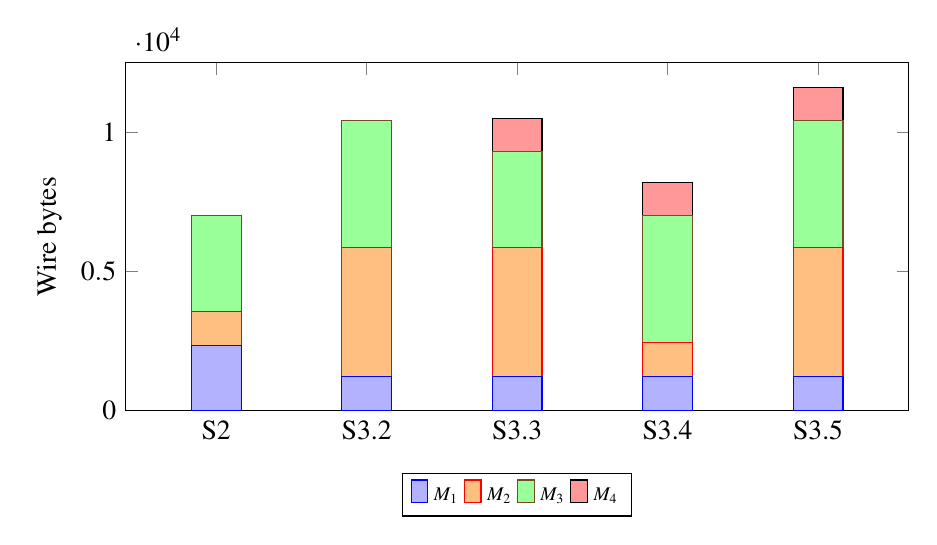
\begin{tikzpicture}
\begin{axis}[
    width=0.95\linewidth, height=6cm,
    ybar stacked, bar width=18pt,
    ymin=0, ymax=12500,
    ylabel={Wire bytes},
    symbolic x coords={S2,S3.2,S3.3,S3.4,S3.5},
    xtick=data,
    legend style={at={(0.5,-0.18)},anchor=north,legend columns=4,font=\scriptsize},
    nodes near coords align={vertical},
    every node near coord/.append style={font=\tiny},
    enlarge x limits=0.15,
]
\addplot+[fill=blue!30] coordinates {(S2,2344)(S3.2,1221)(S3.3,1221)(S3.4,1221)(S3.5,1221)};
\addplot+[fill=orange!50] coordinates {(S2,1226)(S3.2,4633)(S3.3,4633)(S3.4,1226)(S3.5,4633)};
\addplot+[fill=green!40] coordinates {(S2,3461)(S3.2,4577)(S3.3,3461)(S3.4,4577)(S3.5,4577)};
\addplot+[fill=red!40] coordinates {(S2,0)(S3.2,0)(S3.3,1176)(S3.4,1176)(S3.5,1176)};
\legend{$M_1$,$M_2$,$M_3$,$M_4$}
\end{axis}
\end{tikzpicture}
\caption{Per-message contribution to total wire bytes (stacked) for the
five EAP-EDHOC-PQ variants at a 256-byte EAP fragment size.
\VarSecShort{2} pays for $\mathit{kem.ct}_R$ inside $M_1$, while
the four-flight hybrids (\VarSecShort{3.3}, \VarSecShort{3.4},
\VarSecShort{3.5}) add an explicit $M_4$.}
\label{fig:wire-stacked}
\end{figure}
\FloatBarrier
Table~\ref{tab:processing} reports the mean end-to-end handshake time
(in microseconds), broken down by deployment and party. Total
handshake time (Initiator+Responder combined) on the AAA path ranges
from approximately $56$~ms for \VarSec{3.2} to $440$~ms for
\VarSec{3.4}. Two observations stand out. \emph{First}, the AAA path is
never the slowest configuration despite adding a RADIUS hop: for
\VarSec{3.4} and \VarSec{3.5}, the Non-EAP and Standalone paths are
actually slower because they lack the AAA server's optimized
fragment-reassembly primitives. \emph{Second}, \VarSec{3.2} is
dramatically faster than \VarSec{2} in the Initiator/Responder sum
($56$~ms vs.\ $131$~ms on AAA), because \VarSec{2} uses an especially
large Message\,3 ($3{,}461$ bytes) that requires $14$ fragments,
whereas \VarSec{3.2} reuses a compact Message\,1.

\begin{table}[h]
\centering
\footnotesize
\caption{Mean end-to-end processing time per handshake in microseconds
($\mu$s), by deployment and role. ``Sum'' is Initiator+Responder.}
\label{tab:processing}
\begin{tabular}{lrrrrrrrrr}
\toprule
& \multicolumn{3}{c}{\textbf{AAA (FreeRADIUS)}} & \multicolumn{3}{c}{\textbf{EAP-Standalone}} & \multicolumn{3}{c}{\textbf{Non-EAP}} \\
\cmidrule(lr){2-4}\cmidrule(lr){5-7}\cmidrule(lr){8-10}
\textbf{Variant} & Init & Resp & Sum & Init & Resp & Sum & Init & Resp & Sum \\
\midrule
\VarSecShort{2}   &  64{,}505 &  66{,}870 & 131{,}375 &  65{,}621 &  68{,}578 & 134{,}199 &  69{,}038 &  71{,}971 & 141{,}009 \\
\VarSecShort{3.2} &  28{,}051 &  28{,}130 &  56{,}181 &  35{,}668 &  35{,}715 &  71{,}383 &  32{,}133 &  33{,}524 &  65{,}657 \\
\VarSecShort{3.3} & 172{,}086 & 186{,}444 & 358{,}530 & 173{,}831 & 187{,}152 & 360{,}982 & 165{,}068 & 151{,}258 & 316{,}326 \\
\VarSecShort{3.4} & 219{,}917 & 220{,}463 & 440{,}379 & 236{,}108 & 245{,}434 & 481{,}543 & 241{,}271 & 241{,}371 & 482{,}641 \\
\VarSecShort{3.5} & 184{,}496 & 180{,}137 & 364{,}633 & 213{,}043 & 211{,}815 & 424{,}859 & 192{,}235 & 194{,}671 & 386{,}906 \\
\bottomrule
\end{tabular}
\end{table}

% --- Line chart: total handshake time across deployments ---
\begin{figure}[H]
\centering
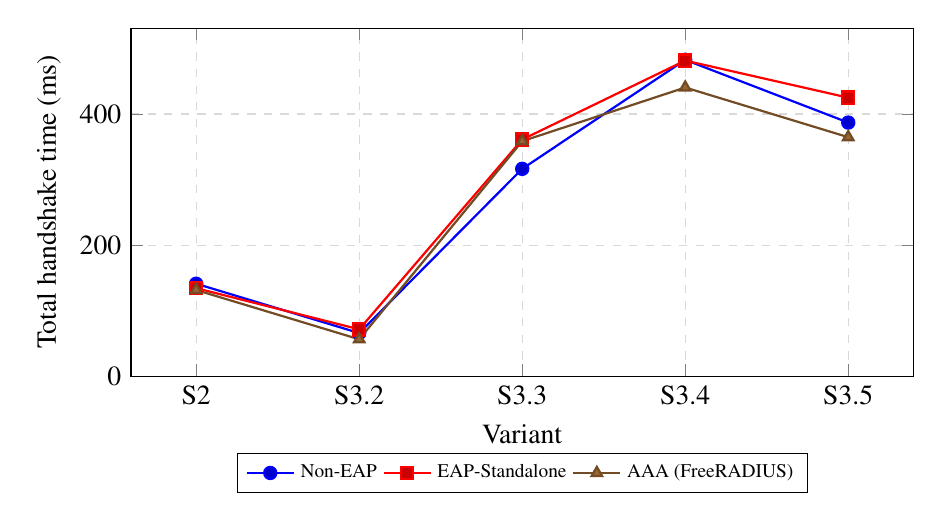
\begin{tikzpicture}
\begin{axis}[
    width=0.95\linewidth, height=6cm,
    ylabel={Total handshake time (ms)},
    xlabel={Variant},
    symbolic x coords={S2,S3.2,S3.3,S3.4,S3.5},
    xtick=data,
    ymin=0,
    legend style={at={(0.5,-0.22)},anchor=north,legend columns=3,font=\scriptsize},
    grid=both, grid style={dashed,gray!30},
    mark options={scale=1.1},
]
\addplot+[mark=*,thick] coordinates {(S2,141.0)(S3.2,65.7)(S3.3,316.3)(S3.4,482.6)(S3.5,386.9)};
\addplot+[mark=square*,thick] coordinates {(S2,134.2)(S3.2,71.4)(S3.3,361.0)(S3.4,481.5)(S3.5,424.9)};
\addplot+[mark=triangle*,thick] coordinates {(S2,131.4)(S3.2,56.2)(S3.3,358.5)(S3.4,440.4)(S3.5,364.6)};
\legend{Non-EAP, EAP-Standalone, AAA (FreeRADIUS)}
\end{axis}
\end{tikzpicture}
\caption{End-to-end handshake time per variant across the three
deployments. Curves cross between three-flight and four-flight
variants; the FreeRADIUS-backed AAA path is competitive with
EAP-Standalone for every variant.}
\label{fig:handshake-line}
\end{figure}
\FloatBarrier
Table~\ref{tab:overhead} reports the decomposition of the wall-clock
handshake time into CPU (compute) time, I/O waiting time
($\mathit{io\_wait}$), and residual overhead (framing, memcpy,
fragmentation state machines). The CPU-to-wall-clock ratio is
consistently below $25\%$ across all variants, which means that the
vast majority of the handshake wall-clock time is spent waiting for
the network and for fragment reassembly --- a direct consequence of
EAP's lock-step fragmentation at 256-byte granularity. RSS peak memory
is around $2.1$--$2.2$~MB for all three deployments, confirming that
the scheme is deployable on typical IoT class~2 devices.

\begin{table}[h]
\centering
\footnotesize
\caption{CPU time, I/O wait, residual overhead, and CPU/wall ratio for
the AAA deployment. All times in microseconds.}
\label{tab:overhead}
\begin{tabular}{llrrrrr}
\toprule
\textbf{Variant} & \textbf{Role} & \textbf{CPU ($\mu$s)} & \textbf{Wall ($\mu$s)} & \textbf{I/O wait} & \textbf{Residual} & \textbf{CPU/Wall} \\
\midrule
\VarSecShort{2}   & Init &  5{,}623 &  64{,}505 &  50{,}103 &   8{,}834 & 0.087 \\
\VarSecShort{2}   & Resp &  1{,}750 &  66{,}870 &   3{,}074 &  62{,}155 & 0.026 \\
\VarSecShort{3.2} & Init &  7{,}029 &  28{,}051 &   7{,}688 &  13{,}405 & 0.251 \\
\VarSecShort{3.2} & Resp &  5{,}929 &  28{,}130 &   1{,}920 &  20{,}482 & 0.211 \\
\VarSecShort{3.3} & Init &  5{,}025 & 172{,}086 &  58{,}156 & 108{,}989 & 0.029 \\
\VarSecShort{3.3} & Resp & 13{,}336 & 186{,}444 & 101{,}110 &  72{,}365 & 0.072 \\
\VarSecShort{3.4} & Init &  5{,}170 & 219{,}917 & 101{,}312 & 113{,}511 & 0.024 \\
\VarSecShort{3.4} & Resp &  6{,}812 & 220{,}463 &  96{,}770 & 117{,}272 & 0.031 \\
\VarSecShort{3.5} & Init & 10{,}252 & 184{,}496 &  58{,}130 & 116{,}219 & 0.056 \\
\VarSecShort{3.5} & Resp & 14{,}866 & 180{,}137 &  86{,}543 &  79{,}184 & 0.083 \\
\bottomrule
\end{tabular}
\end{table}

% --- Horizontal stacked bar: CPU vs IO-wait vs residual per (variant,role) ---
\begin{figure}[H]
\centering
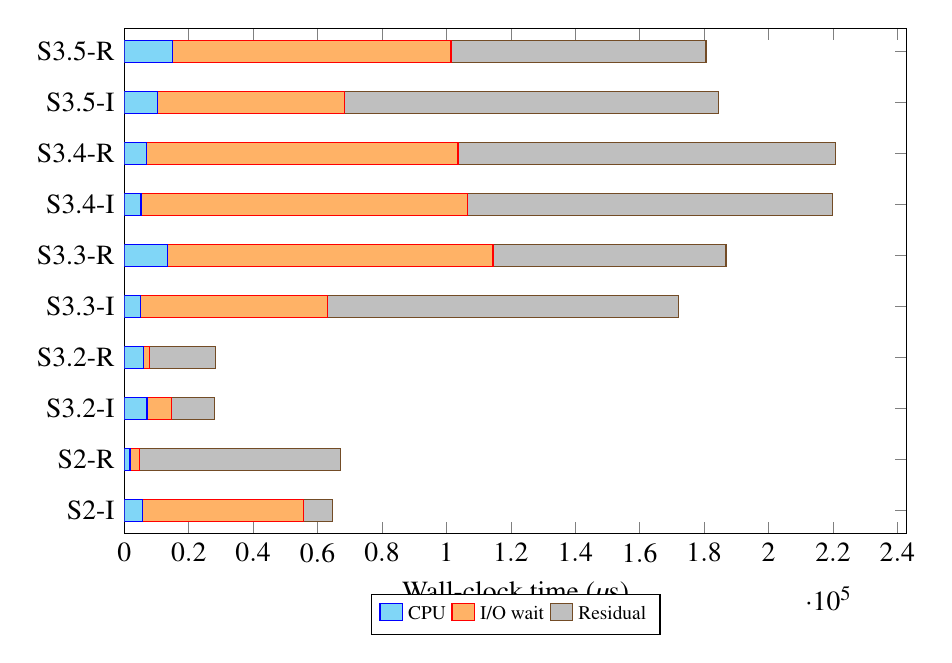
\begin{tikzpicture}
\begin{axis}[
    width=0.95\linewidth, height=8cm,
    xbar stacked, bar width=8pt,
    xmin=0,
    xlabel={Wall-clock time ($\mu$s)},
    symbolic y coords={S2-I,S2-R,S3.2-I,S3.2-R,S3.3-I,S3.3-R,S3.4-I,S3.4-R,S3.5-I,S3.5-R},
    ytick=data,
    legend style={at={(0.5,-0.12)},anchor=north,legend columns=3,font=\scriptsize},
    enlarge y limits=0.05,
    every axis plot/.append style={draw=black!40},
]
\addplot+[fill=cyan!50] coordinates {
  (5623,S2-I)(1750,S2-R)(7029,S3.2-I)(5929,S3.2-R)
  (5025,S3.3-I)(13336,S3.3-R)(5170,S3.4-I)(6812,S3.4-R)
  (10252,S3.5-I)(14866,S3.5-R)};
\addplot+[fill=orange!60] coordinates {
  (50103,S2-I)(3074,S2-R)(7688,S3.2-I)(1920,S3.2-R)
  (58156,S3.3-I)(101110,S3.3-R)(101312,S3.4-I)(96770,S3.4-R)
  (58130,S3.5-I)(86543,S3.5-R)};
\addplot+[fill=gray!50] coordinates {
  (8834,S2-I)(62155,S2-R)(13405,S3.2-I)(20482,S3.2-R)
  (108989,S3.3-I)(72365,S3.3-R)(113511,S3.4-I)(117272,S3.4-R)
  (116219,S3.5-I)(79184,S3.5-R)};
\legend{CPU, I/O wait, Residual}
\end{axis}
\end{tikzpicture}
\caption{Wall-clock breakdown into CPU, I/O wait, and residual
overhead for each (variant, role) on the AAA deployment. The CPU
bands are uniformly thin: cryptography is dwarfed by fragmentation
latency in every configuration.}
\label{fig:overhead-stacked}
\end{figure}
\FloatBarrier
Table~\ref{tab:operations} reports the total time per handshake spent
in each primitive operation, measured on the AAA deployment.
Signature generation is by far the largest cryptographic contributor
(typically $2{,}165$--$8{,}822$ $\mu$s per invocation) and dominates
the cryptographic budget for every variant that uses ML-DSA. ML-KEM
$\KemKeyGen$, $\Encaps$, and $\Decaps$ are comparatively cheap, each
in the $230$--$2{,}035$~$\mu$s range. Across every variant,
cryptography accounts for substantially less than the fragment-induced
I/O wait, reinforcing the conclusion from Table~\ref{tab:overhead}
that \emph{fragmentation, not cryptography, dominates EAP-EDHOC-PQ's
wall-clock cost under the 256-byte fragment regime.}

\begin{table}[h]
\centering
\footnotesize
\caption{Total per-handshake cryptographic time (in $\mu$s) on the AAA
deployment. Dash (---) indicates operation not invoked by the variant
on that role.}
\label{tab:operations}
\begin{tabular}{llrrrrrrr}
\toprule
\textbf{Variant} & \textbf{Role} & \textbf{KeyGen} & \textbf{Encaps} & \textbf{Decaps} & \textbf{Sign} & \textbf{Verify} & \textbf{HKDF} & \textbf{AEAD} \\
\midrule
\VarSecShort{2}   & Init & 370 &    472 &  608 & 4{,}067 & ---       &  20 &  13 \\
\VarSecShort{2}   & Resp & 232 &    283 &  345 & ---     &    697    &  17 &  46 \\
\VarSecShort{3.2} & Init & 374 &    470 &  609 & 4{,}337 &    943    & 205 &   9 \\
\VarSecShort{3.2} & Resp & 376 &    413 &  631 & 2{,}830 & 1{,}181   & 225 &  56 \\
\VarSecShort{3.3} & Init & 370 & ---    & 1{,}215 & 2{,}165 &    942 & 210 &  10 \\
\VarSecShort{3.3} & Resp & 805 & 1{,}520 & ---    & 8{,}822 & 1{,}380 & 310 &  72 \\
\VarSecShort{3.4} & Init & 371 &    470 & 1{,}218 & 2{,}968 & ---     &  25 &  11 \\
\VarSecShort{3.4} & Resp & 731 & 1{,}776 & 1{,}234 & ---     & 2{,}424 &  75 & 112 \\
\VarSecShort{3.5} & Init & 371 &    473 & 1{,}223 & 6{,}885 &    943  & 211 &  11 \\
\VarSecShort{3.5} & Resp & 906 & 2{,}034 & 1{,}224 & 7{,}163 & 2{,}445 & 445 & 118 \\
\bottomrule
\end{tabular}
\end{table}

% --- Polar / radar plot: per-operation cost shape per variant (Responder) ---
\begin{figure}[H]
\centering
\begin{tikzpicture}
\begin{polaraxis}[
    width=0.85\linewidth, height=8cm,
    xtick={0,51.43,...,308.57},
    xticklabels={KeyGen,Encaps,Decaps,Sign,Verify,HKDF,AEAD},
    ymin=0, ymax=10000,
    ytick={2000,4000,6000,8000},
    yticklabel style={font=\tiny},
    xticklabel style={font=\tiny},
    legend style={at={(1.25,1.0)},anchor=north west,font=\scriptsize},
]
% S2 (Resp): 232,283,345,0,697,17,46
\addplot+[mark=*] coordinates {(0,232)(51.43,283)(102.86,345)(154.29,0)(205.71,697)(257.14,17)(308.57,46)(360,232)};
% S3.2: 376,413,631,2830,1181,225,56
\addplot+[mark=square*] coordinates {(0,376)(51.43,413)(102.86,631)(154.29,2830)(205.71,1181)(257.14,225)(308.57,56)(360,376)};
% S3.3: 805,1520,0,8822,1380,310,72
\addplot+[mark=triangle*] coordinates {(0,805)(51.43,1520)(102.86,0)(154.29,8822)(205.71,1380)(257.14,310)(308.57,72)(360,805)};
% S3.4: 731,1776,1234,0,2424,75,112
\addplot+[mark=diamond*] coordinates {(0,731)(51.43,1776)(102.86,1234)(154.29,0)(205.71,2424)(257.14,75)(308.57,112)(360,731)};
% S3.5: 906,2034,1224,7163,2445,445,118
\addplot+[mark=pentagon*] coordinates {(0,906)(51.43,2034)(102.86,1224)(154.29,7163)(205.71,2445)(257.14,445)(308.57,118)(360,906)};
\legend{S2,S3.2,S3.3,S3.4,S3.5}
\end{polaraxis}
\end{tikzpicture}
\caption{Per-operation cryptographic cost (Responder side, AAA
deployment), drawn as a radar plot. Variants relying on ML-DSA
(\VarSecShort{3.3} and \VarSecShort{3.5}) extend along the
\textsc{Sign} spoke; \VarSecShort{3.4} extends along
\textsc{Encaps}/\textsc{Decaps}/\textsc{Verify} instead.}
\label{fig:ops-radar}
\end{figure}
\FloatBarrier

%-------------------------------------------------------------------------
\subsection{Energy Consumption}
\label{sec:energy}
%-------------------------------------------------------------------------
Wall-clock measurements alone do not capture the impact of EAP
fragmentation on \emph{battery-operated} IoT endpoints, which
dominate e-business deployments such as wireless vending machines and
battery-powered sensor nodes. We therefore use the per-handshake
timings of Table~\ref{tab:overhead} to derive a transparent,
first-order energy estimate. We adopt a deliberately simple model so
that the assumptions are auditable; we do not claim sub-mJ accuracy.

\paragraph{Model.} For one handshake we approximate the per-role
energy as the sum of three additive components,
\begin{equation}
E_{\mathrm{hs}} \;=\; P_{\mathrm{cpu}}\cdot t_{\mathrm{cpu}}
\;+\; P_{\mathrm{idle}}\cdot t_{\mathrm{io}}
\;+\; P_{\mathrm{tx}}\cdot \frac{8\,B_{\mathrm{wire}}}{R_{\mathrm{tx}}},
\label{eq:energy}
\end{equation}
where $t_{\mathrm{cpu}}$ is the CPU time of
Table~\ref{tab:overhead}, $t_{\mathrm{io}}$ is the I/O-wait time of
the same table, $B_{\mathrm{wire}}$ are the per-role wire bytes of
Table~\ref{tab:frag}, and $R_{\mathrm{tx}}$ is the link bit-rate.
Reference power values are typical of an ARM Cortex-M class IoT node
with a low-power radio:
$P_{\mathrm{cpu}}\!=\!48$~mW (active),
$P_{\mathrm{idle}}\!=\!4$~mW (MCU light-sleep waiting on the radio),
$P_{\mathrm{tx}}\!=\!60$~mW (radio in TX/RX), and
$R_{\mathrm{tx}}\!=\!250$~kbps (IEEE~802.15.4-class throughput).
These values are within the range reported by widely-cited IoT
characterizations~\cite{FVW24,FTK+25} and are stated explicitly so
that the table can be re-scaled by the reader for a different
platform: under~\eqref{eq:energy}, $E_{\mathrm{hs}}$ scales linearly
in every $P_*$ and inversely in $R_{\mathrm{tx}}$.

\paragraph{Results.} Table~\ref{tab:energy} reports the per-role
energy estimate using \eqref{eq:energy} on the AAA deployment. The
total per-handshake energy ranges from $\approx\!4$~mJ for
\VarSecShort{3.2} to $\approx\!22$~mJ for \VarSecShort{3.4}, and the
share attributable to CPU is at most $\approx\!13\%$. The dominant
share is the I/O-wait term, confirming at the energy level the
fragmentation-bound conclusion already drawn from
Table~\ref{tab:overhead}.

\begin{table}[H]
\centering
\footnotesize
\caption{First-order per-handshake energy estimate from
\eqref{eq:energy} on the AAA deployment, in millijoules. Reference
parameters: $P_{\mathrm{cpu}}\!=\!48$~mW, $P_{\mathrm{idle}}\!=\!4$~mW,
$P_{\mathrm{tx}}\!=\!60$~mW, $R_{\mathrm{tx}}\!=\!250$~kbps.
$E_{\mathrm{cpu}}\!=\!P_{\mathrm{cpu}} t_{\mathrm{cpu}}$,
$E_{\mathrm{io}}\!=\!P_{\mathrm{idle}} t_{\mathrm{io}}$,
$E_{\mathrm{tx}}\!=\!P_{\mathrm{tx}}\!\cdot\!8B_{\mathrm{wire}}/R_{\mathrm{tx}}$.
Wire bytes are split per role using Table~\ref{tab:frag} ($M_1,M_3$
from $I$, $M_2,M_4$ from $R$).}
\label{tab:energy}
\begin{tabular}{llrrrr}
\toprule
\textbf{Variant} & \textbf{Role} & $E_{\mathrm{cpu}}$ (mJ) & $E_{\mathrm{io}}$ (mJ) & $E_{\mathrm{tx}}$ (mJ) & $E_{\mathrm{hs}}$ (mJ) \\
\midrule
\VarSecShort{2}   & Init & 0.27 & 0.20 & 1.11 &  1.58 \\
\VarSecShort{2}   & Resp & 0.08 & 0.01 & 0.24 &  0.33 \\
\VarSecShort{3.2} & Init & 0.34 & 0.03 & 1.11 &  1.48 \\
\VarSecShort{3.2} & Resp & 0.28 & 0.01 & 0.89 &  1.18 \\
\VarSecShort{3.3} & Init & 0.24 & 0.23 & 0.90 &  1.37 \\
\VarSecShort{3.3} & Resp & 0.64 & 0.40 & 1.12 &  2.16 \\
\VarSecShort{3.4} & Init & 0.25 & 0.41 & 1.11 &  1.77 \\
\VarSecShort{3.4} & Resp & 0.33 & 0.39 & 0.46 &  1.18 \\
\VarSecShort{3.5} & Init & 0.49 & 0.23 & 1.11 &  1.83 \\
\VarSecShort{3.5} & Resp & 0.71 & 0.35 & 1.12 &  2.18 \\
\midrule
\VarSecShort{2}   & Sum  & 0.35 & 0.21 & 1.35 &  1.91 \\
\VarSecShort{3.2} & Sum  & 0.62 & 0.04 & 2.00 &  2.66 \\
\VarSecShort{3.3} & Sum  & 0.88 & 0.63 & 2.02 &  3.53 \\
\VarSecShort{3.4} & Sum  & 0.58 & 0.80 & 1.57 &  2.95 \\
\VarSecShort{3.5} & Sum  & 1.20 & 0.58 & 2.23 &  4.01 \\
\bottomrule
\end{tabular}
\end{table}

% --- Grouped bar: per-role energy split (CPU vs IO vs TX) ---
\begin{figure}[H]
\centering
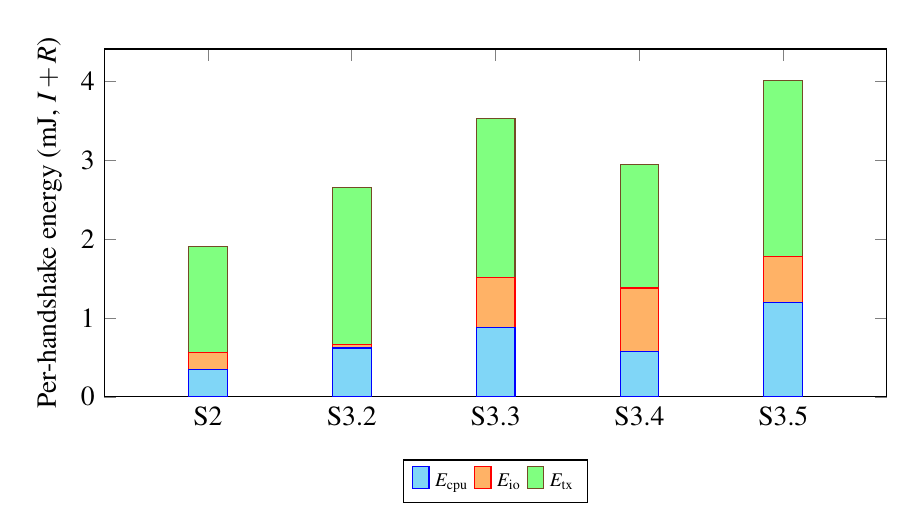
\begin{tikzpicture}
\begin{axis}[
    width=0.95\linewidth, height=6cm,
    ybar stacked, bar width=14pt,
    ymin=0,
    ylabel={Per-handshake energy (mJ, $I+R$)},
    symbolic x coords={S2,S3.2,S3.3,S3.4,S3.5},
    xtick=data,
    legend style={at={(0.5,-0.18)},anchor=north,legend columns=3,font=\scriptsize},
    enlarge x limits=0.18,
]
\addplot+[fill=cyan!50] coordinates {(S2,0.35)(S3.2,0.62)(S3.3,0.88)(S3.4,0.58)(S3.5,1.20)};
\addplot+[fill=orange!60] coordinates {(S2,0.21)(S3.2,0.04)(S3.3,0.63)(S3.4,0.80)(S3.5,0.58)};
\addplot+[fill=green!50] coordinates {(S2,1.35)(S3.2,2.00)(S3.3,2.02)(S3.4,1.57)(S3.5,2.23)};
\legend{$E_{\mathrm{cpu}}$,$E_{\mathrm{io}}$,$E_{\mathrm{tx}}$}
\end{axis}
\end{tikzpicture}
\caption{Per-handshake energy estimate ($I\!+\!R$) under
\eqref{eq:energy}. The transmit term $E_{\mathrm{tx}}$ tracks the
stacked wire bytes of Fig.~\ref{fig:wire-stacked}, while the CPU
contribution remains a minor share for every variant.}
\label{fig:energy-stacked}
\end{figure}
\FloatBarrier


%=========================================================================
\section{Discussion}
\label{discussion}
%=========================================================================
Our results lead to several observations of practical consequence.

\paragraph{Fragmentation, not cryptography, drives wall-clock time.}
Across every variant and every deployment, the CPU-to-wall-clock ratio
stays below~$0.25$. The I/O wait time spent on fragment ACKs alone
accounts for $50$--$60\%$ of the total handshake time for the
four-flight variants. Bumping the EAP fragment size above $1024$
bytes --- which is already allowed by RFC~3748 when the lower layer
supports it --- would mechanically cut the fragment count by a factor
of four, and we conjecture would reduce wall-clock handshake time
proportionally.

\paragraph{Deferred Responder authentication (\texorpdfstring{\VarSec{3.4}}{Section 3.4}) is attractive.}
Despite being a four-flight hybrid with the largest Message\,3
($4{,}577$ bytes), \VarSec{3.4} keeps total wire bytes to $8{,}207$
and total fragments to~$34$, substantially smaller than \VarSec{3.2},
\VarSec{3.3}, and \VarSec{3.5}. The price is that the Initiator cannot
accept the Responder's authentication until Message\,4. For EAP
network access this is a benign trade-off: the EAP-Success is sent
only after Message\,4 in any case.

\paragraph{\texorpdfstring{\VarSec{2}}{Section 2} is the right default for KEM-trusting environments.}
If the deployment already distributes the Responder's KEM public key
(e.g., via a pre-provisioned onboarding credential), \VarSec{2}
produces the smallest wire footprint and uses a single ML-DSA
signature (instead of two), for a clean three-flight handshake that
maps natively onto EAP's request/response pattern.

\paragraph{AAA does not necessarily slow things down.}
Contrary to intuition, the FreeRADIUS-backed AAA deployment is not the
slowest one in our measurements; for \VarSec{3.4} it is in fact
$\sim\!10\%$ faster than EAP-Standalone. We attribute this to
FreeRADIUS's efficient RADIUS packetization and its batched I/O path,
which compensates for the extra RADIUS hop. This is an encouraging
result for production deployments.

\paragraph{Energy follows the wire, not the CPU.}
The first-order energy model of Section~\ref{sec:energy} ranks the
five variants in essentially the same order as their wire-byte and
fragment-count totals: $E_{\mathrm{tx}}$ and $E_{\mathrm{io}}$
together dominate $E_{\mathrm{cpu}}$ for every variant
(Table~\ref{tab:energy}). For battery-operated e-business endpoints
such as wireless vending terminals or asset trackers, this means
that picking a smaller-on-the-wire variant (\VarSecShort{2} or
\VarSecShort{3.4}) yields a larger battery payoff than picking a
cryptographically lighter primitive at the same parameter level.

\paragraph{Limitations and future work.}
Our measurements use ML-KEM-768/ML-DSA-44 and a 256-byte fragment
size; evaluating Level\,3 and Level\,5 parameter sets, larger fragment
sizes, and lossy wireless lower layers (e.g., 802.15.4, LoRaWAN) is
left for future work. Our ProVerif model treats ML-KEM as an idealized
IND-CCA2 KEM; a computational analysis along the lines
of~\cite{Fer24,GM23} remains open.


%=========================================================================
\section{Conclusion}
\label{conclusion}
%=========================================================================
We have presented EAP-EDHOC-PQ, a unified specification that brings
the five post-quantum authentication modes of EDHOC --- \VarSec{2},
\VarSec{3.2}, \VarSec{3.3}, \VarSec{3.4} and \VarSec{3.5} --- to the
EAP framework, and we have evaluated it formally in ProVerif and
empirically over Non-EAP, EAP-Standalone, and FreeRADIUS-backed AAA
deployments. All five variants satisfy mutual authentication,
session-key secrecy, forward secrecy, and replay resistance.
Empirically, \VarSec{3.2} is the fastest three-flight variant,
\VarSec{2} is the smallest on the wire, and \VarSec{3.4} offers the
best trade-off among four-flight hybrid modes thanks to its deferred
Responder authentication. A first-order energy model derived from the
same measurements shows that the per-handshake energy budget on a
typical IoT-class node is dominated by transmission and I/O wait
rather than by cryptography, so optimizing the negotiated EAP
fragment size is a more impactful lever for future PQ-EAP methods
than accelerating the underlying KEM. These findings, while limited
to the parameter sets and link rates we measured, chart a practical
starting point for quantum-resistant network access authentication of
Wi-Fi-attached IoT endpoints in e-business deployments such as
networked vending machines, smart-retail beacons, and connected
logistics sensors.


\label{sect:bib}
\bibliographystyle{unsrt}
\bibliography{reference}

\end{document}